\chapter{\textit{CP} parameters measurement}

The measurement of $\it{CP}$ parameters $\mathcal{S}$ and $\mathcal{A}$ are perform by fitting  Equation \ref{eq:tdcpv_sig} to the distribution of events with respect to the decay time difference $\Delta t$ and flavor $q$, where $\Delta t = t_{CP}-t_{tag}$ and $q =  +1(-1)$ when the tag-side $B$ meson is $B^0$($\bar{B^0}$). 

\begin{equation}\label{eq:tdcpv_sig}
\mathcal{P}_{sig}(\Delta t, q ) = 
\frac{e^{-|\Delta t|/\tau_{B^0}}}{4\tau_{B^0}}
\begin{Bmatrix}
1 + q \cdot 
\begin{bmatrix}
\mathcal{S}sin(\Delta M_d \Delta t) + 
\mathcal{A}cos(\Delta M_d \Delta t)
\end{bmatrix}
\end{Bmatrix}
\end{equation}

The Equation \ref{eq:tdcpv_sig} describes the physics distribution of signal events only. To perform the unbinned maximum likelihood fit on data, a complete model for \textit{i}-th event that includes the overlay of background components and outlier bands can be defined as Equation \ref{eq:tdcpv_all}.

\begin{equation}\label{eq:tdcpv_all}
\begin{split}
\mathcal{P}(\Delta t_i,q_i,f_i^{sig},\mathcal{S},\mathcal{A})
&=(1-f_{ol})\begin{bmatrix}f_{sig}\mathcal{P}_{sig}(\Delta t_i,q_i,\mathcal{S},\mathcal{A})+(1-f_{sig}\mathcal{P}_{bkg}(\Delta t_i))
\end{bmatrix}\\
&+f_{ol}\mathcal{P}_{ol}(\Delta t_i)
\end{split}
\end{equation}

where $f_{sig}$ and $f_{ol}$ are the fraction of signal and outlier components, respectively. The $\mathcal{P}_{bkg}$ and $\mathcal{P}_{ol}$ are defined by Equation \ref{eq:p_bkg} and \ref{eq:p_out}.

\begin{equation}\label{eq:p_bkg}
\mathcal{P}_{bkg} (\Delta t_i)=
f_{bkg}^{\delta}\delta(\Delta t_i-\mu_{bkg}^{\delta})+(1-f_{bkg}^{\delta})
\frac{1}{2\tau_{bkg}}e^{-|\Delta t_i-\mu_{\tau}^{bkg}|/\tau_{bkg}}
\end{equation}

\begin{equation}\label{eq:p_out}
\mathcal{P}_{ol} (\Delta t_i)=
G(\Delta t_i, \sigma_{ol})
\end{equation}

where $\delta(\Delta t_i-\mu_{bkg}^{\delta})$ is Dirac $\delta$ function and $G$ is single Gaussian. The outlier component is to improve the fit quality with large $\Delta t$ events.

\section{Vertex Resolution Model}

The Equation \ref{eq:tdcpv_all} presents an ideal distribution of $\Delta t_i$ for each event without considering the difference between measured and the true position of the vertex. The difference can be described by introducing resolution functions, turning Equation \ref{eq:tdcpv_all} into Equation \ref{eq:tdcpv_all_res}.
\begin{equation}\label{eq:tdcpv_all_res}
\begin{split}
\mathcal{P}(\Delta t_i,q_i,f_i^{sig},\mathcal{S},\mathcal{A})
&=(1-f_{ol})\text{[}f_{sig}\mathcal{P}_{sig}(\Delta t_i)\otimes R_{sig}(\Delta t_i)\\
&+(1-f_{sig})\mathcal{P}_{bkg}(\Delta t_i)\otimes R_{bkg}(\Delta t_i)
\text{]}\\
&+f_{ol}\mathcal{P}_{ol}(\Delta t_i)\otimes R_{ol}(\Delta t_i)
\end{split}
\end{equation}

The $R_{sig}$ stands for the resolution function for signal events, which receives smearing effect from \textit{CP} and tag side separately, namely $R_{cp}$ and  $R_{tag}$. The treatment of \textit{CP} side and tag side is different because of vertexing strategies. For \textit{CP} side, vertex of $B^0$ is reconstructed by fully fitting all the daughter particles. Instead, in tag side, there's no full reconstruction of $B^0$ so vertex fit is applied for the selected charged tracks in the rest-of-event. The background events have its own resolution model which is independent from  $\it{CP}$ violation parameters. The outlier is used to smooth fit for large $\Delta t$ events. In the low statistics case as the current luminosity is, the outlier is not included in the fit to have a more realistic model for data.

For signal events, the resolution functions are studied for $\it{CP}$-side and tag-side based on each possible degradation such as detector resolutions, effect of tracks from non-primary $B$ vertex and so on. Such a method is used in Belle analysis and named as artificial model. Details are summarized in \cite{Yusa-note}. Considered the vertex position difference $\Delta z$ for signal events as shown in Equation \ref{eq:dz}. 

\begin{equation}\label{eq:dz}
\Delta z 
=\Delta z^{'} + (z_{cp}^{}- z_{cp}^{'}) - (z_{tag}^{}- z_{tag}^{'}) 
\end{equation}where the primed ones stands for physics truth of the position and the non-primed is the measured value, the resolution function receives contribution from both $\it{CP}$ and tag-side effects. In the meantime, the resolution functions on both sides also depend on the applied constraint. Considering that the fine structure of IP profile is not yet fully understood and small discrepancies have been observed between data and simulation\cite{jpsiks_ichep}, there's no IP constraint applied for both sides in vertex fit, which avoids potential bias from  IP profile under this low statistical situation. The combined contributions can be presented as Equation \ref{eq:Rsig}.

\begin{equation}\label{eq:Rsig}
R_{sig}=R_{cp}\otimes R_{tag}
\end{equation}

\subsection{$\it{CP}$-side resolution function}

$\it{CP}$-side vertex is fitted with all tracks from a reconstructed $B^0$, thus the resolution models only depend on detectors' effect. For each event, the resolution effect can be different based on event-by-event reconstruction quality, primarily presented by the reduced $\chi^2$ called $\chi^2/N$ from \textit{TreeFit}, which $N$ is the degree of freedom of the fit. The distribution of $\chi^2/N$ in data are shown in Figure \ref{fig:redchi2}. 

\begin{figure}[H]
	\centering
	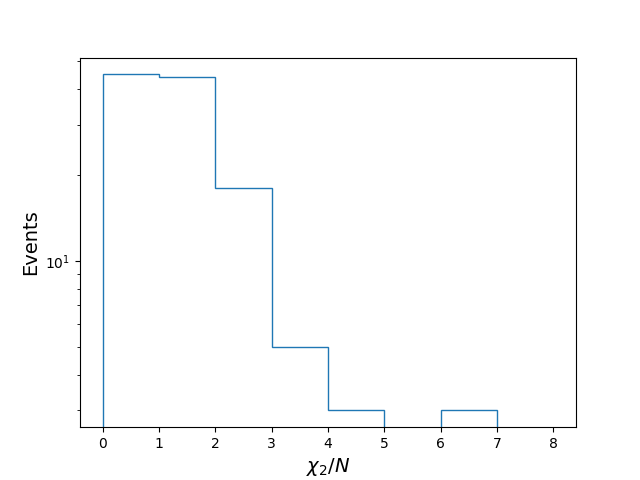
\includegraphics[height=6cm]{redChi2.png}
	\caption{$\chi^2/N$ of selected events from data.}
	\label{fig:redchi2}
\end{figure}

Therefore, we model the resolution functions on $\it{CP}$-side by using a double Gaussian function, where the mean is fixed to zero and the standard deviation is scaled by $\chi^2/N$ and the error of reconstructed vertex $\sigma_{z_{cp}}$, as shown in Equation \ref{eq:Rcp}.
\begin{equation}\label{eq:Rcp}
R_{cp}(\delta z_{cp}) = (1-f_{cp}^{tail})G(0,s_{cp}^{main})+
f_{cp}^{tail}G(0,s_{cp}^{tail})
\end{equation} where $s_{cp}^{main}$ and $s_{cp}^{tail}$ are defined in Equation \ref{eq:scp_mt}.
\begin{eqnarray}\label{eq:scp_mt}
\begin{split}
s_{cp}^{main}&=(s_0^{main} + s_1^{main}\cdot \chi^2_{cp}/N )\cdot \sigma_{z_{cp}}\\
s_{cp}^{tail}&=(s_0^{tail} + s_1^{tail}\cdot \chi^2_{cp}/N )\cdot \sigma_{z_{cp}}
\end{split}
\end{eqnarray} 
The dependence of resolution models on $\chi^2/N$ is shown in Figure \ref{fig:redchi2fit}. Restrictively speaking, the $\it{CP}$-side resolution for $B^0 \to K_S^0  K_S^0  K_S^0$ is slight different from $B^0\to J/\psi K_S^0$, due to the absence of the direct charged tracks from the $B^0$ vertex. The modification of the resolution function on $\it{CP}$-side will be further studied when more data becomes available in future. Given the current low statistics, the Equation \ref{eq:Rcp} works well as an approximation. By fitting the resolution function using \textit{signal MC} on $\it{CP}$-side, the parameters are fitted which are listed in Table \ref{tab:Rcp}.
\begin{figure}[htbp]
	\begin{subfigure}{0.5\linewidth}
		\caption{$0<\chi^2/N<10$}
		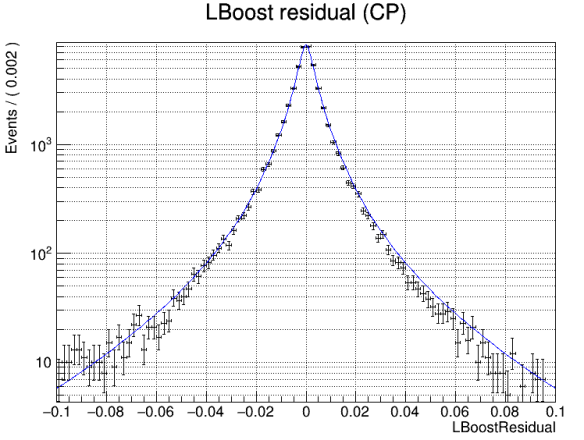
\includegraphics[height=5cm]{figures/residual0_10}
		
	\end{subfigure}
	\begin{subfigure}{0.5\linewidth}
		\caption{$0<\chi^2/N<0.4$}
		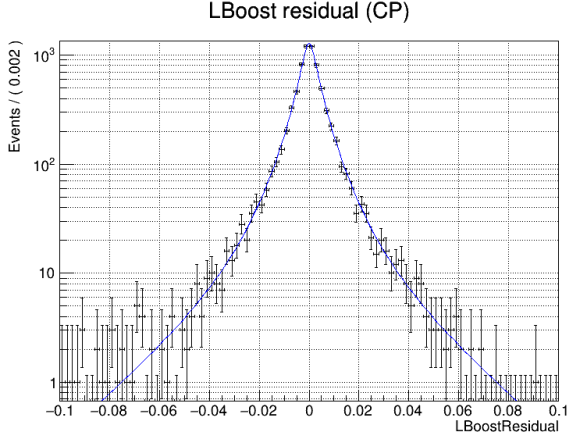
\includegraphics[height=5cm]{figures/residual0_0.4}
		%\caption{Tagging efficiency $\epsilon$ and $\mu$ in r-bins for $B^0 \to K_S^0  K_S^0  K_S^0$.}
	\end{subfigure}
	
	
	\begin{subfigure}{0.5\linewidth}
		\caption{$0.4<\chi^2/N<0.8$}
		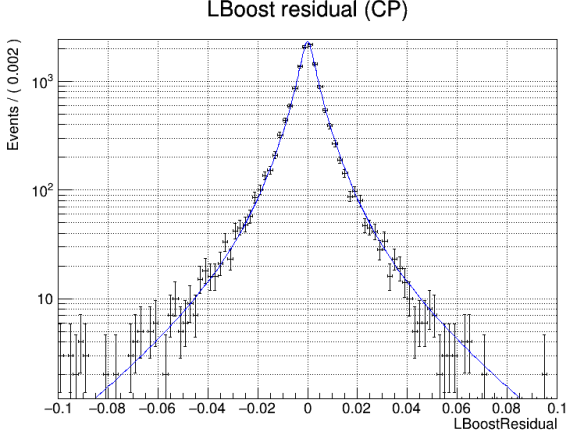
\includegraphics[height=5cm]{figures/residual0.4_0.8}
		%\caption{Tagging efficiency $\epsilon$ and $\mu$ in r-bins for $B^0 \to K_S^0  K_S^0  K_S^0$.}
	\end{subfigure}
	\begin{subfigure}{0.5\linewidth}
		\caption{$0.8<\chi^2/N<1.2$}
		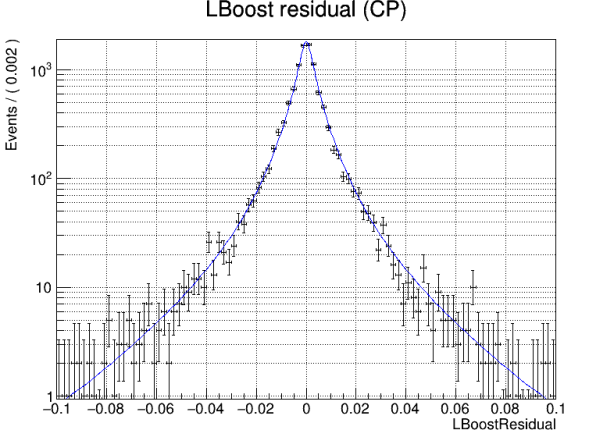
\includegraphics[height=5cm]{figures/residual0.8_1.2}
		%\caption{Tagging efficiency $\epsilon$ and $\mu$ in r-bins for $B^0 \to K_S^0  K_S^0  K_S^0$.}
	\end{subfigure}
	
	\begin{subfigure}{0.5\linewidth}
		\caption{$1.2<\chi^2/N<1.6$}
		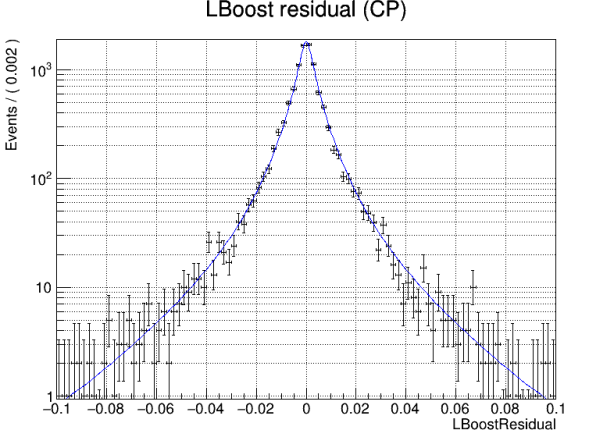
\includegraphics[height=5cm]{figures/residual1.2_1.6}
		%\caption{Tagging efficiency $\epsilon$ and $\mu$ in r-bins for $B^0 \to K_S^0  K_S^0  K_S^0$.}
	\end{subfigure}
	\begin{subfigure}{0.5\linewidth}
		\caption{$1.6<\chi^2/N<10$}
		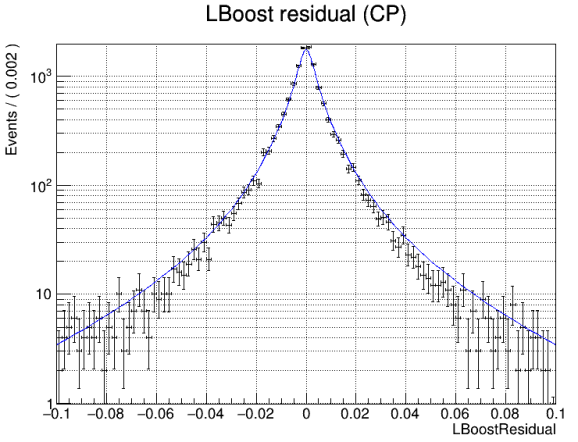
\includegraphics[height=5cm]{figures/residual1.6_10}
		%\caption{Tagging efficiency $\epsilon$ and $\mu$ in r-bins for $B^0 \to K_S^0  K_S^0  K_S^0$.}
	\end{subfigure}
	\caption{Resolution functions on $\it{CP}$-side, which shows dependence on the $\chi^2/N$}
	\label{fig:redchi2fit}
\end{figure}

\begin{table}[H]
	\begin{minipage}[b]{1.0\linewidth}
		\centering
		\caption{Parameters in $R_{cp}$.}
		\label{tab:Rcp}
		\begin{tabular}{|c|c|}
			\hline
			$f_{cp}^{tail}$ & $0.07424 \pm 0.0008$\\
			$s_0^{main}$&  $0.9151 \pm 0.0077$ \\
			$s_1^{main}$ & $0.2142\pm 0.0064$\\
			$s_0^{tail}$ &  $2.0477\pm 0.0779$\\
			$s_1^{tail}$  & $1.3470\pm 0.0720$ \\
			\hline
		\end{tabular}
	\end{minipage}
\end{table}

\subsection{Tag-side resolution function}

For the tag-side, the vertexing is done by using \textit{KFit} and no IP constraint used. Due to the charged tracks from non-primary $B$ vertex, the resolution functions on tag-side not only receives contribution from detectors' effect $R_{det}^{tag}$ but also the resolution degradation from secondary vertex, called $R_{np}^{tag}$. To the contrary, if all tracks that are used for tag-side vertexing are primary tracks, the resolution will only be affected by the detectors' effect. The vertex position difference is defined as Equation \ref{eq:ztag}. Therefore, the effects from both detectors and non-primary tracks contributes to the total resolution on tag-side as Equation \ref{eq:Rtag} shows.
\begin{equation}\label{eq:ztag}
\begin{split}
z_{tag} - z_{tag}^{'} =& (z_{tag}^{'} + \delta z_{tag}^{det} + \delta z_{tag}^{np}) - z_{tag}^{'}\\
=&\delta z_{tag}^{det} + \delta z_{tag}^{np}
\end{split}
\end{equation}
\begin{equation}\label{eq:Rtag}
R_{tag}( z_{tag}- z_{tag}^{'}) = R_{det}^{tag}(\delta z_{tag}^{det}) \otimes
R_{np}^{tag}( \delta z_{tag}^{np})
\end{equation}

Similarly to $\it{CP}$-side resolution function, detectors' effect is presented in Equation \ref{eq:Rtagdet}
\begin{equation}\label{eq:Rtagdet}
R_{det}^{tag}(\delta z_{tag}^{det}) = (1-f_{tag}^{tail})G(0,s_{tag}^{main}\cdot\sigma_{z_{tag}})+
f_{tag}^{tail}G(0,s_{tag}^{tail}\cdot\sigma_{z_{tag}})
\end{equation} where main and tail Gaussian functions have the same central value at zero, but the standard deviation is scaled by $\chi^2_{tag}/N$ on the tag-side as shown in Equation \ref{eq:stag}.

\begin{equation}\label{eq:stag}
s_{tag}^{main/tail} = s_0^{main/tail} + s_1^{main/tail}\cdot\chi^2_{tag}/N
\end{equation} 
Technically $R^{tag}_{det}$ can be fitted with MC samples of which tag-side tracks are all from primary vertex. After obtaining the fitted parameters of $R^{tag}_{det}$ , $R^{tag}$ will only be dependent on $R^{tag}_{np}$. The fit model of $R_{np}^{tag}$ is shown in Equation \ref{eq:Rnp}. It consists of three functions, including one Dirac $\delta$ function and two single-side exponential functions $E_p$ and $E_n$. The $E_p(x,\tau_p)=(1/\tau_p)e^{-x/\tau_p} $ when $x > 0$ and the $E_n(x,\tau_n)=(1/\tau_n)e^{x/\tau_n} $ when $x < 0$.
The exponential factors in both positive and negative components are scaled by the tag-side vertex uncertainty $\sigma_{z_{tag}}$. 

\begin{equation}\label{eq:Rnp}
R_{np}^{tag}(\delta z_{tag}^{np})=f_{\delta}\delta(\delta z_{tag}^{np}) + 
(1-f_{\delta})[f_p E_p(\delta z_{tag}^{np},\tau_p\cdot \sigma_{z_{tag}}) +
(1-f_p)E_n(\delta z_{tag}^{np},\tau_n\cdot \sigma_{z_{tag}}) ]
\end{equation} 


Also, since tag-side has no dependence on how $\it{CP}$-side is reconstructed, the resolution functions on tag-sdie are almost mode-independent. Thus these parameters are obtained by fitting to the control sample data. The details about control sample study are here\cite{jpsiks_ichep}. The fit plots for tag-side resolution functions are shown in Figure \ref{fig:Rtagdet} and \ref{fig:Rtagnp}. The parameters obtained from the fit are listed in Table \ref{tab:Rtagdet} and Table \ref{tab:Rtagnp}.


\begin{figure}[H]
	\begin{minipage}[b]{0.5\linewidth}
		\centering
		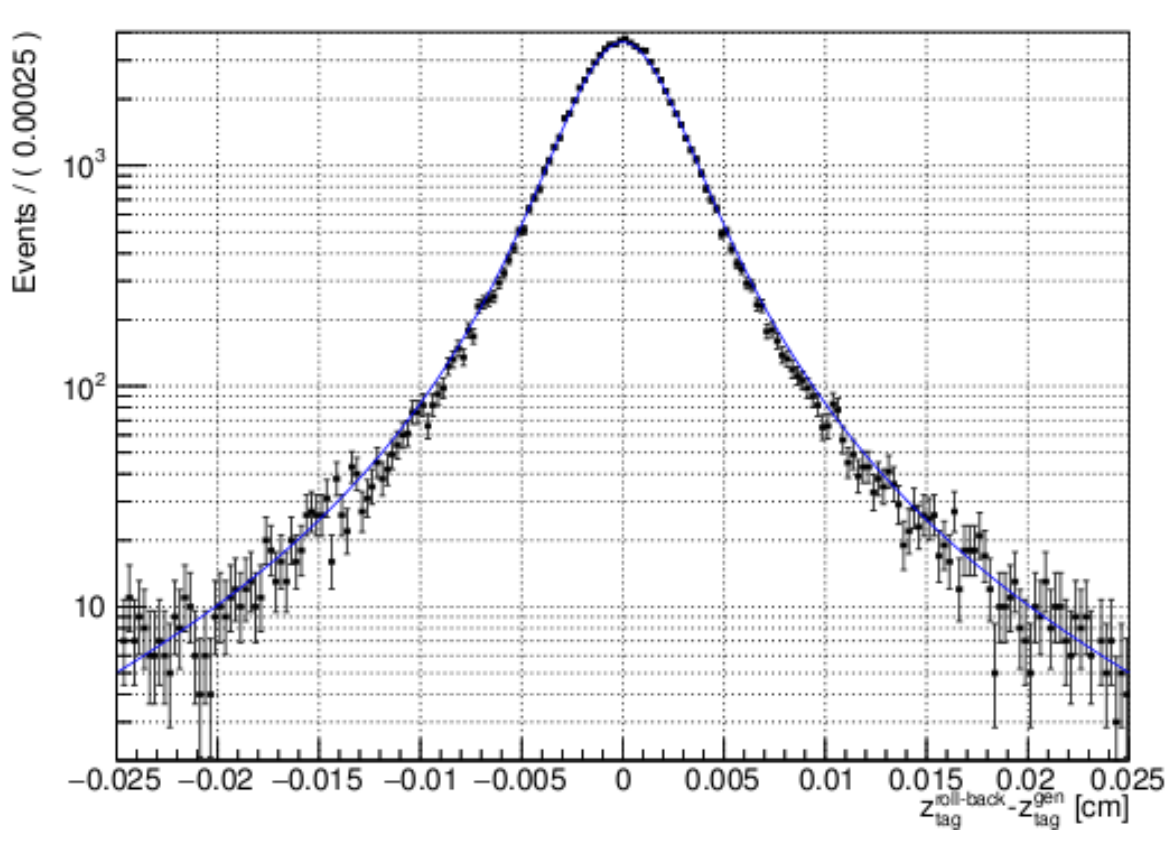
\includegraphics[height=5cm]{figures/Rdet}
		\caption{$R_{det}^{tag} $ fit}
		\label{fig:Rtagdet}
	\end{minipage}
	\begin{minipage}[b]{0.5\linewidth}
		\centering
		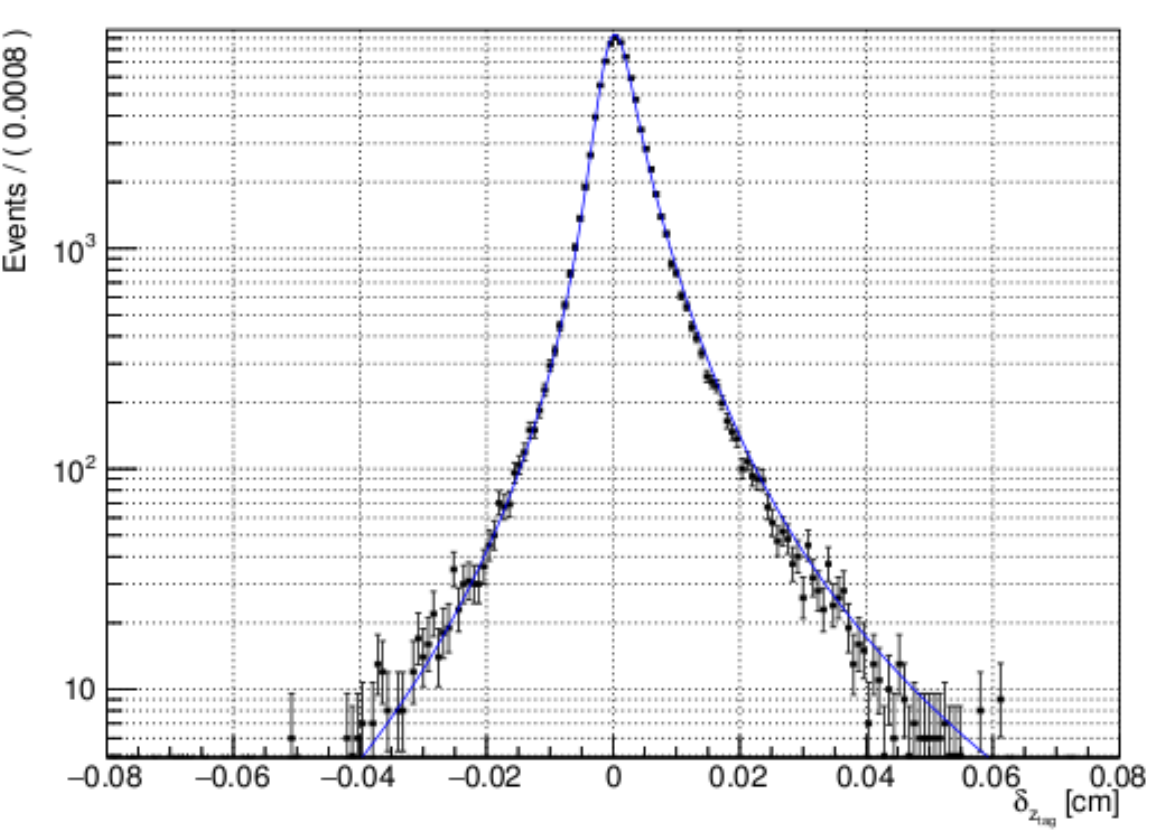
\includegraphics[height=5cm]{figures/Rnp}
		\caption{$R_{np}^{tag}$ fit}
		\label{fig:Rtagnp}
	\end{minipage}
\end{figure}

\begin{table}[H]
	\begin{minipage}[b]{0.5\linewidth}
		\centering
		\caption{Parameters in $R^{tag}_{det}$}
		\label{tab:Rtagdet}
		\begin{tabular}{|c|c|}
			\hline
			$f_{tag}^{tail}$ & $0.0523 \pm 0.0025$\\
			$s_0^{main}$&  $1.1446 \pm 0.0061$ \\
			$s_1^{main}$ & $0.0443\pm 0.0022$\\
			$s_0^{tail}$ &  $3.4480\pm 0.0897$\\
			$s_1^{tail}$  & $0.2666\pm0.0276$ \\
			\hline
		\end{tabular}
	\end{minipage}
	\begin{minipage}[b]{0.5\linewidth}
		\centering
		\caption{Parameters in $R^{tag}_{np}$}
		\label{tab:Rtagnp}
		\begin{tabular}{|c|c|}
			\hline
			$f_{\delta}$ & $0.6256\pm 0.0049$\\
			$f_p$ &  $0.8316 \pm 0.0051$ \\
			$\tau_n$ & $2.9141\pm 0.0758$\\
			$\tau_p$ &  $2.4846\pm 0.0269$\\
			\hline
		\end{tabular}
	\end{minipage}
\end{table}


 The boost direction of each event is not constant event-by-event, so the position of vertex may not be optimized by calculating $\Delta t_i = \Delta z / \beta\gamma c$. This effect can be reduced by replacing vertex position difference on z-axis with the relative distance along the boosting direction, or introducing another resolution function called $R_k$\cite{tajima2004proper}. The $R_k$ has not been implemented in Belle II resolution model. Therefore, $\Delta z$ projection on the boosted direction of each event is used for reducing this kinematics effect on resolution function.



\subsection{Background events $\Delta t$ distribution}
The $R_{bkg}$ is uncorrelated to vertex reconstruction method approximately. Because the background mainly comes from continuum events passing the selection, it's reasonable to model its resolution by a Gaussian-like function. A double-Gaussian with its standard deviation scaled by the measured uncertainties from both sides is used as Equation \ref{eq:Rbkg}. To be noted, unlike resolution functions on $\it{CP}$ or tag-side, the standard deviations of the double Gaussian are scaled by both the vertex position uncertainties $\sigma_{z_{cp}}$ and $\sigma_{z_{tag}}$. 

\begin{equation}\label{eq:Rbkg}
R_{bkg} = (1-f^{bkg}_{tail})G(\Delta t_i, \sigma^{bkg}_{main}\sqrt{\sigma^2_{z_{cp}}+\sigma^2_{z_{tag}}})
+ f^{bkg}_{tail}G(\Delta t_i, \sigma^{bkg}_{tail}\sqrt{\sigma^2_{z_{cp}}+\sigma^2_{z_{tag}}})
\end{equation}

The background events $\Delta t$ shapes $\mathcal{P}_{bkg}\otimes R_{bkg}$ can be determined by fitting to side-band data. There are totally seven floating parameters which are listed in Table  \ref{tab:Pbkg} with fitted values using 60 sideband events at $M_{bc} < 5.26$ GeV, shown in Figure \ref{fig:Pbkg}

\begin{figure}[htpb]
	%	\begin{minipage}[b]{0.5\linewidth}
	%		\centering
	%		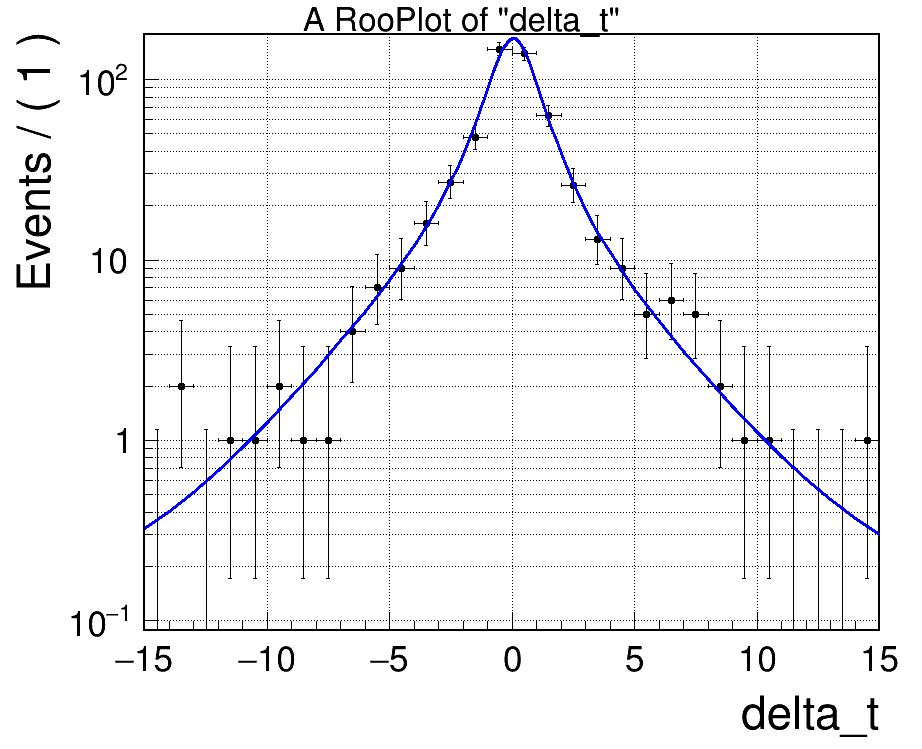
\includegraphics[height=5cm]{figures/bkg-cpfit-gen-mbc526}
	%		\caption{Background fit on generic sideband}
	%	\end{minipage}
	%	\begin{minipage}[b]{0.5\linewidth}
	\centering
	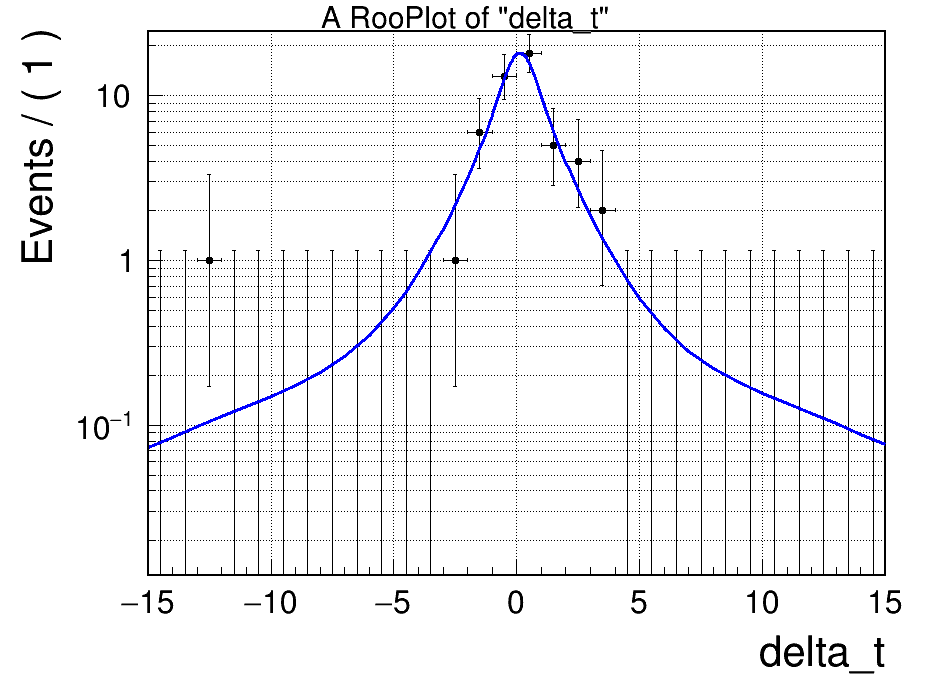
\includegraphics[height=5cm]{figures/bkg-cpfit-data-mbc526}
	\caption{$\mathcal{P}_{bkg}\otimes R_{bkg}$ fit  using 60 sideband events at $M_{bc} < 5.26$ GeV.}
	\label{fig:Pbkg}
	%	\end{minipage}
\end{figure}
\begin{table}[H]
	\centering
	\begin{tabular}{|c|c|}
		\hline
		$\mu^{bkg}_{\delta}$ & $0.1310 \pm 0.1902$\\
		$\mu^{bkg}_{l}$&  $0.1638 \pm 0.5030$ \\
		$\tau_{bkg}$ & $1.0541\pm 0.4370$\\
		$f_{\delta}^{bkg}$ &  $0.5861\pm 0.2570$\\
		$f^{bkg}_{tail}$  & $0.0417\pm 0.0408$ \\
		$\sigma^{bkg}_{main}$ & $1.4348\pm 0.3940$\\
		$\sigma^{bkg}_{tail}$ & $28.0930 \pm 8.8221$\\
		\hline
	\end{tabular}
	\caption{Parameters in Background $\Delta t$ distribution. }
	\label{tab:Pbkg}
\end{table}


\section{Flavor Tagging}
 In order to determine the flavor of tag side $B^0$, flavor tagging algorithm is being developed. The flavor tagging uses information from $\mu^{\pm}$, $\pi^{\pm}$,$K^{\pm}$ and $\Lambda^{}$ which are categorized into 13 different types as illustrated in Figure \ref{fig:flavortagger}. 

\begin{figure}[H]
\centering
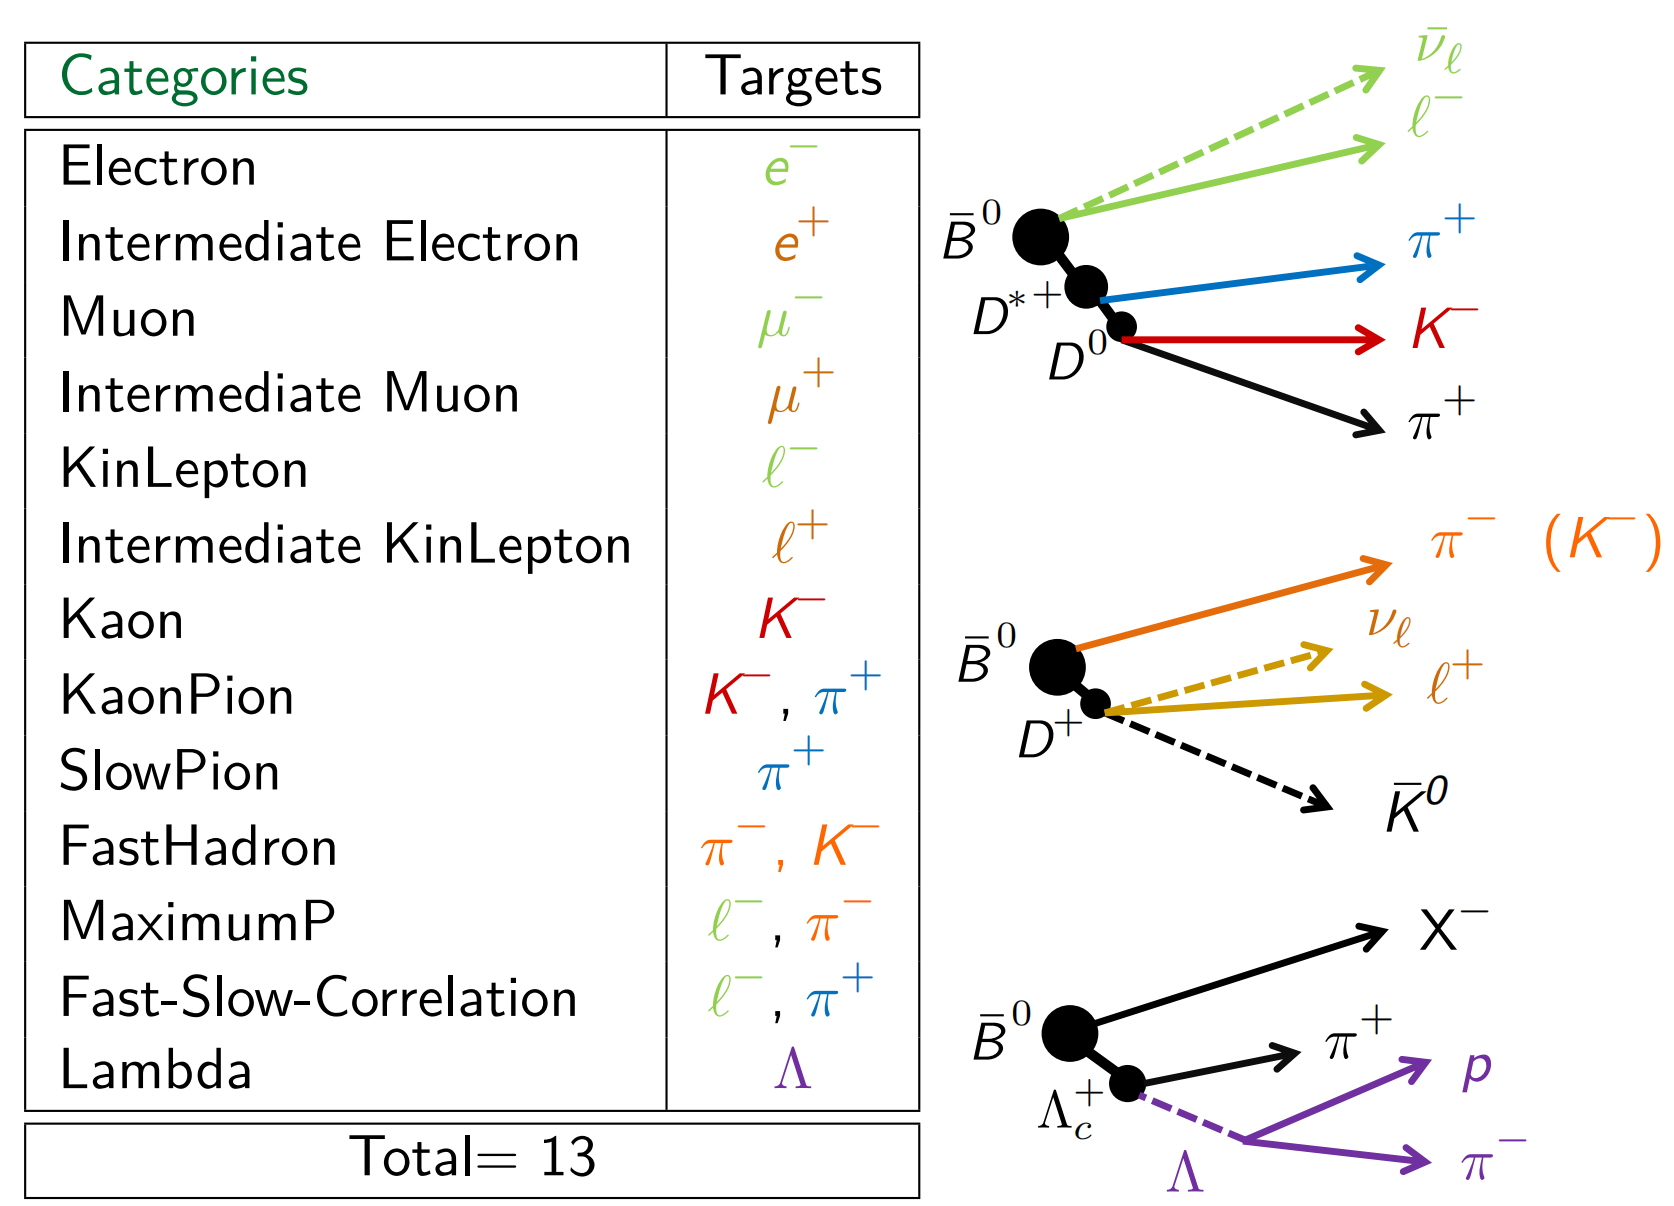
\includegraphics[width=0.7\linewidth]{tagger}
\caption{Particles and their categories used in flavor tagging algorithm\cite{flavortagger}.}
\label{fig:flavortagger}
\end{figure}
 
 
For each particle that has been used from above categories, PID and kinematics information are extracted and feed to the combiner as training variables, to obtained a classifier response corresponding to each category. Then for all responses from these categories, a total classifier is trained to present the likelihood of flavor $q$. This algorithm is called category-based method and used in this thesis. After the reconstruction on the \textit{CP}-side $B^0$ is done, the rest-of-events tracks used to form the particle lists are selected\ref{fig:flavortagger}. The FastBDT as the back-end algorithm is chosen for performing training on the classifier of flavor tagging. Targeted variable is true $q$ of tag-side neutral $B$ in MC. To minimize impact of the reconstruction performance on $\it{CP}$-side, MC sample of $B^0 \to \nu \nu$ is used as the training sample where the final state in $\it{CP}$-side are completely invisible. 

Considering the limited power of flavor tagging accuracy, there is a certain fraction of events that are wrongly tagged among all that can be flavor tagged using the final state particles in the rest-of-event. Thus, the flavor tagging efficiency $\epsilon$ and wrong tag fraction $w$ are defined, respectively. Taking into account of the performance of flavor tagging, the observed distribution of Equation \ref{eq:tdcpv_all} becomes Equation \ref{eq:tdcpv_all_ft}.

\begin{equation}\label{eq:tdcpv_all_ft}
\small
\mathcal{P}_{sig}^{obs}(\Delta t, q, \epsilon, w) = 
\frac{e^{-|\Delta t|/\tau_{B^0}}}{4\tau_{B^0}}
\epsilon
\begin{Bmatrix}
1 - q\cdot \Delta w+ q(1-2w)\cdot 
\begin{bmatrix}
\mathcal{S}sin(\Delta M_d \Delta t) + 
\mathcal{A}cos(\Delta M_d \Delta t)
\end{bmatrix}
\end{Bmatrix}
\end{equation} 
Compared to the original, the term with $\mathcal{S}$ and $\mathcal{A}$ is scaled by factor $r\equiv |1-2w|$, defined as the dilution factor. The statistical uncertainty of $\mathcal{S}$ now becomes dependent to the tagging efficiency $\epsilon$ and wrong tag fraction $w$. The uncertainty of $w$ is much larger than $\epsilon$ which makes $w$ an important source of systematic uncertainty, too. The validation of flavor tagger using flavor specific decay modes in 2019 Belle II data is summarized here\cite{abudinen2020first}. The $w$ for each single event is defined as a probability of being wrongly flavor tagged which can be presented by the average wrong tag fraction in a binned interval of the dilution factor. The binned values of dilution factor $r$ is defined for the calculation of $w$ as $[0.0, 0.1, 0.25, 0.5, 0.625, 0.75, 0.875, 1.0]$, also named as $r$-bin. For all events that have been successful tagged, they are projected into histogram of $r$-bin, and $w$ is calculated in each bin by the fraction of events with $q\cdot r$ opposite to its MC flavor. The distribution of $q\cdot r$ is shown in Figure \ref{fig:ft_qr} using \textit{signal MC} of $B^0 \to K_S^0  K_S^0  K_S^0$. 

Besides, $w$ can be different between $B^0$ and $\overline{B^0}$, where
$\bar{w} = (w_{B^0}+w_{\overline{B^0}})/2$ and $\Delta w = w_{B^0}-w_{\overline{B^0}}$. Due to the small value of $\Delta w$, the contribution from $\Delta w$ is treated as zero in Equation \ref{eq:tdcpv_all_ft} in this analysis. Similarly, for $\epsilon$, the values calculated based on each $r$-bin are summed and used in Equation \ref{eq:tdcpv_all_ft}, where the total efficiency is $(99.72\pm0.02)\%$, treated as 1 therefore. The difference $\mu = \epsilon_{B^0}-\epsilon_{\overline{B^0}} $ is about 1 \% to 2 \% in each $r$-bin, thus treated as zero. The distributions of $w$, $\Delta w$, $\epsilon$, and $\mu$ in each $r$-bin are shown in Figure \ref{fig:ft_wtag}.
 \begin{figure}[H]
 	\centering
 	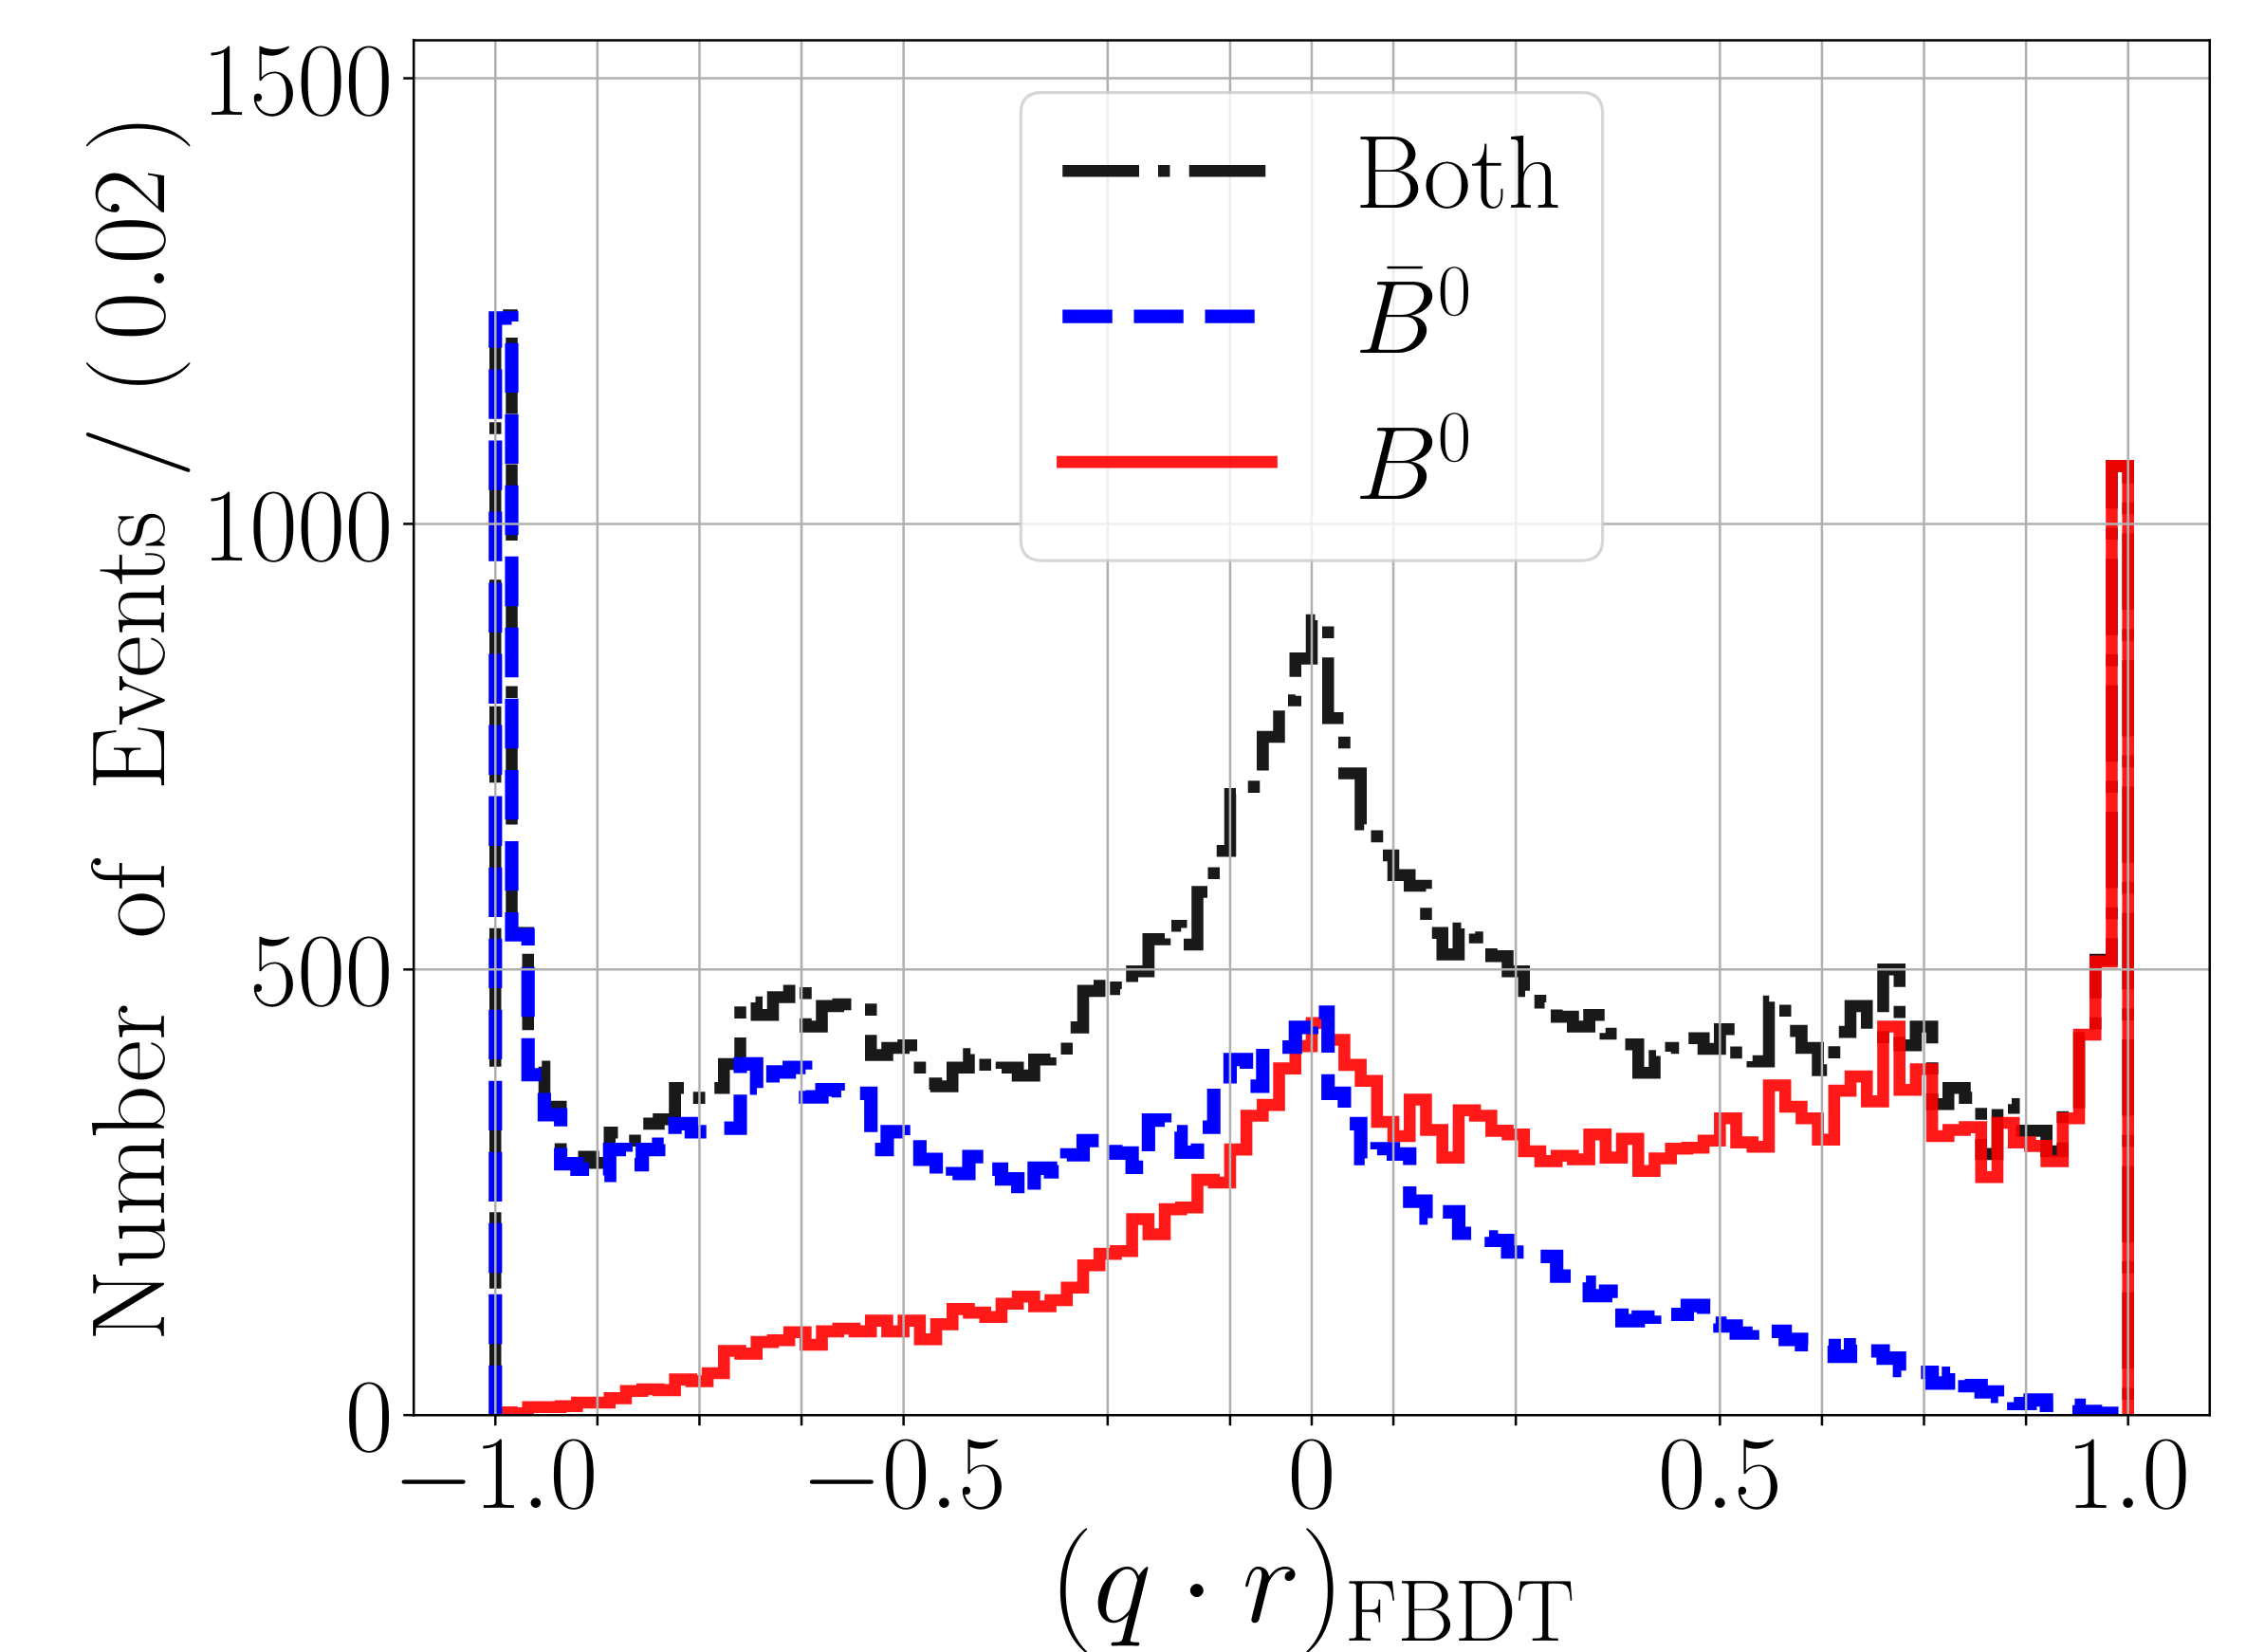
\includegraphics[width=0.7\linewidth]{figures/qr}
 	\caption{The distribution of flavor tagger output $(q\cdot r)$ for both tag-side of $B^0$ and $\overline{B^0}$}
 	\label{fig:ft_qr}
 	\end{figure}
 \begin{figure}[htpb]
 	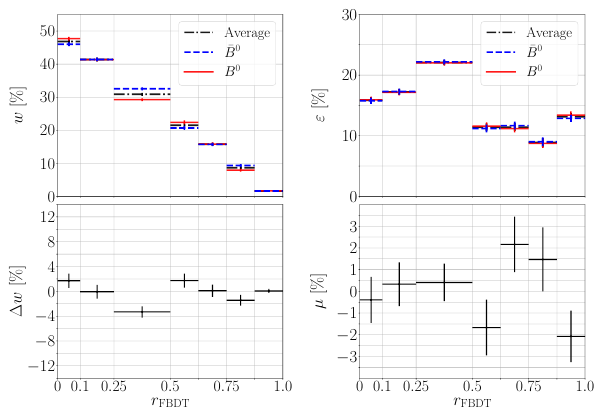
\includegraphics[height=9cm]{flavor_values}
 	\caption{The flavor tagging efficiency, wrong tagging fraction, and their difference between different flavors sorted in each $r$-bin.}
 	\label{fig:ft_wtag}
 \end{figure}

\section{$\it{CP}$ Fitter}

The parameters that are needed for measuring $\mathcal{S}$ and $\mathcal{A}$ are studied and obtainable. Using observed $\Delta t$ distribution from selected events, Equation \ref{eq:tdcpv_all_res} can be fitted using unbinned maximum likelihood fit which takes $\Delta t$, signal fraction $f_{sig}$, the flavor charge $q$ as observables. In the meantime the vertexing error $\sigma_{z_{cp}}$, $\sigma_{z_{tag}}$ and $\chi^2/N$ are used as event-by-event conditional variables that are accessed during the fitting.
For Belle II, a new $\it{CP}$ fitter is developed based on Python and RooFit, which is naturally easy to use and maintained with BASF2. The fitter requires a configuration files which contains all the parameters' definitions including their ranges, initial values, floating states and uncertainties. 

\begin{comment}
\begin{figure}[H]
\centering
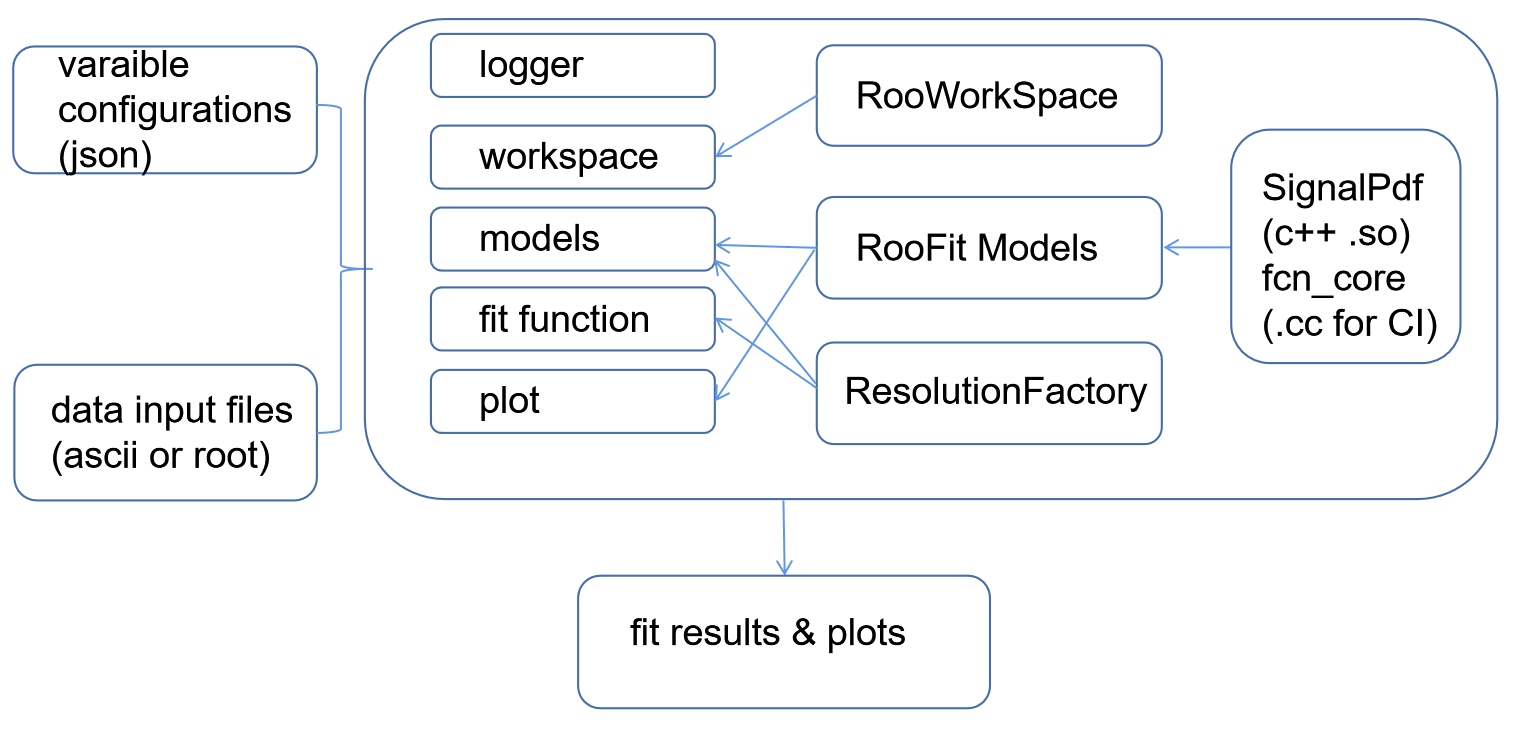
\includegraphics[height=6cm]{cpfitter-pict}
\caption{The structure of $\it{CP}$ fitter for Belle II. Users provide configuration file containing the definitions of all parameters and observables in the $\it{CP}$ fit. Data input files are used to create dataset for fitting. External library called ``SignalPdf.cxx" are generated in runtime to calculate the integral of resolutions and physics distribution event by event, which the fit is performed by maximizing the ``fcn\_core" function, presenting the likelihood of the dataset to the fit model. }
\end{figure}
\end{comment}



%2021/02/11 mid
\section{Blind analysis and fit}
As a required procedure to make sure the $\it{CP}$ parameters are measured without bias due to the preconceived results, a blind analysis procedure is conducted before the fit is actually performed using the experimental data. The blind fit procedure includes the $\it{CP}$ fit on \textit{signal MC} and \textit{generic MC}, with different number of events used. To check the reliablity of fit result from $\it{CP}$ fitter, a linearity test and toy MC study are also performed. 

\subsection{$\it{CP}$ fit on MC samples}
Using $\it{CP}$ fitter, we first perform the $\it{CP}$ fit on events in \textit{signal MC} and \textit{generic MC}.
The \textit{signal MC} and \textit{generic MC} are generated with phase-space model which contains zero $\it{CP}$ violation ($\mathcal{S}=\mathcal{A}=0$). The events that pass the selections in Table \ref{tab:cutCP} are used for $\it{CP}$ parameters fit.
\begin{table}
	\centering
\begin{tabular}{c|c}
	\hline
	Observables & Selections \\
	$\Delta t$ & $-70 < \Delta t < 70$ ps\\
	$\it{CP}$-side $\chi^2/N$ & $0 < (\chi^2/N)_{cp} < 8 $ \\
	tag-side $\chi^2/N$  & $0 < (\chi^2/N)_{tag} < 50 $\\
	$\sigma_{z_{tag}}$ &  $\sigma_{z_{tag}} < 0.1$ cm\\
	signal region & $5.27 < M_{bc} < 5.29$ GeV and $|\Delta E| < 0.1$ GeV\\
	\hline

\end{tabular}
\caption{The selection criteria for events that are used for $\it{CP}$ parameters fit.}
\label{tab:cutCP}
\end{table}



We have 10000 (8873 passing selections) events from signal sample and 415 (373 passing selections) events from 1 ab$^{-1}$ \textit{generic MC} to fit $\it{CP}$ parameters. To mimic the events number expected in data sample, 30 events randomly taken from \textit{generic MC} are used to perform the fit as well. The plots are shown in Figure \ref{fig:cpfit_sig}, \ref{fig:cpfit_gen} and \ref{fig:cpfit_gen_data}. The fit results of $\mathcal{S}$ and $\mathcal{A}$ are summarized in Table \ref{tab:cpfit_result_mc}.
\begin{figure}[H]
	\begin{minipage}{0.5\linewidth}
		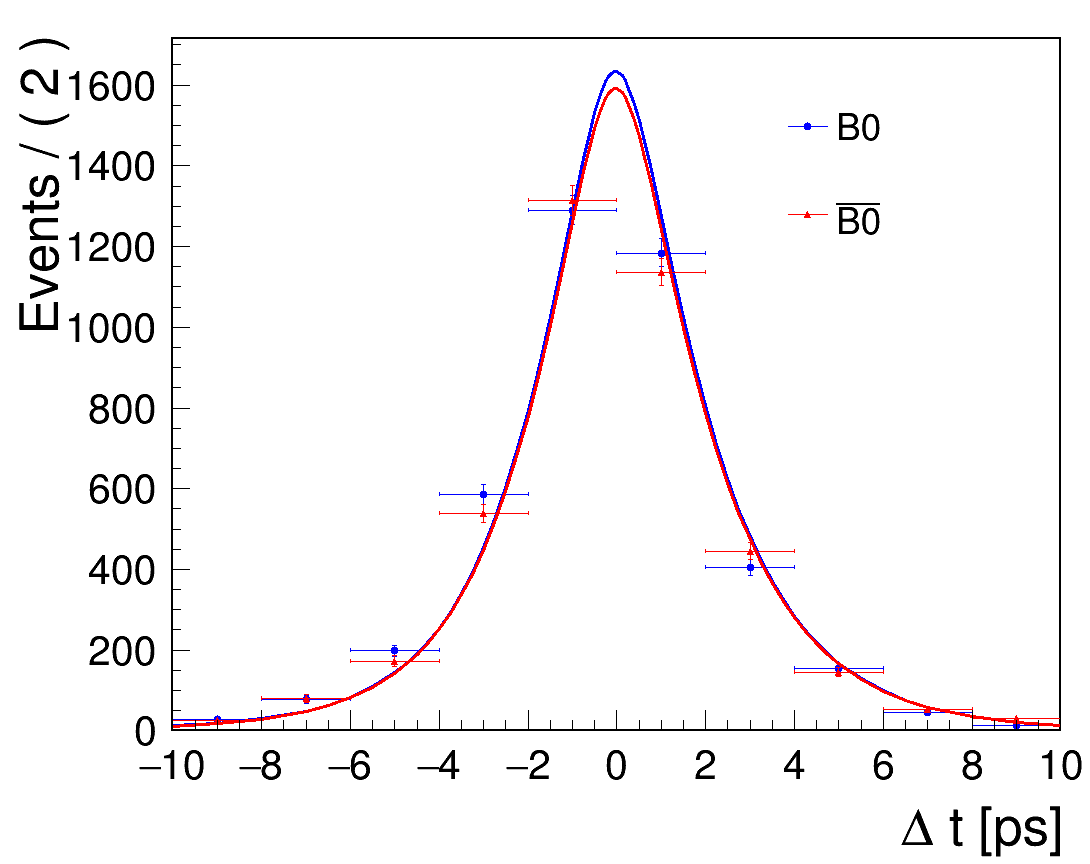
\includegraphics[height=5cm]{figures/cpfit-10000sig}
		\caption{$\it{CP}$ fit on 8873 \textit{signal MC}.}
		\label{fig:cpfit_sig}
	\end{minipage}
	\begin{minipage}{0.5\linewidth}
		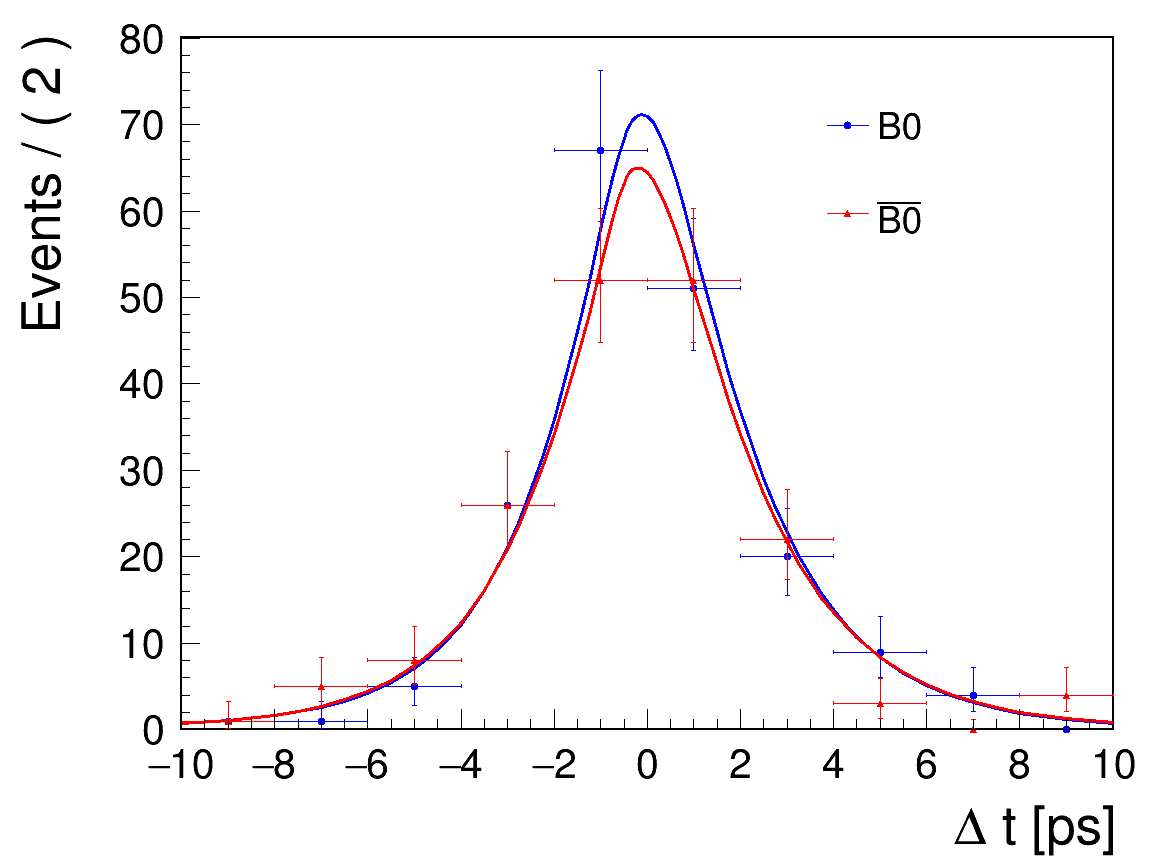
\includegraphics[height=5cm]{figures/cpfit-373gen}
		\caption{$\it{CP}$ fit on 373 \textit{generic MC}.}
		\label{fig:cpfit_gen}
	\end{minipage}
\vspace{0.5cm}
	\begin{minipage}{1\linewidth}
		\centering
		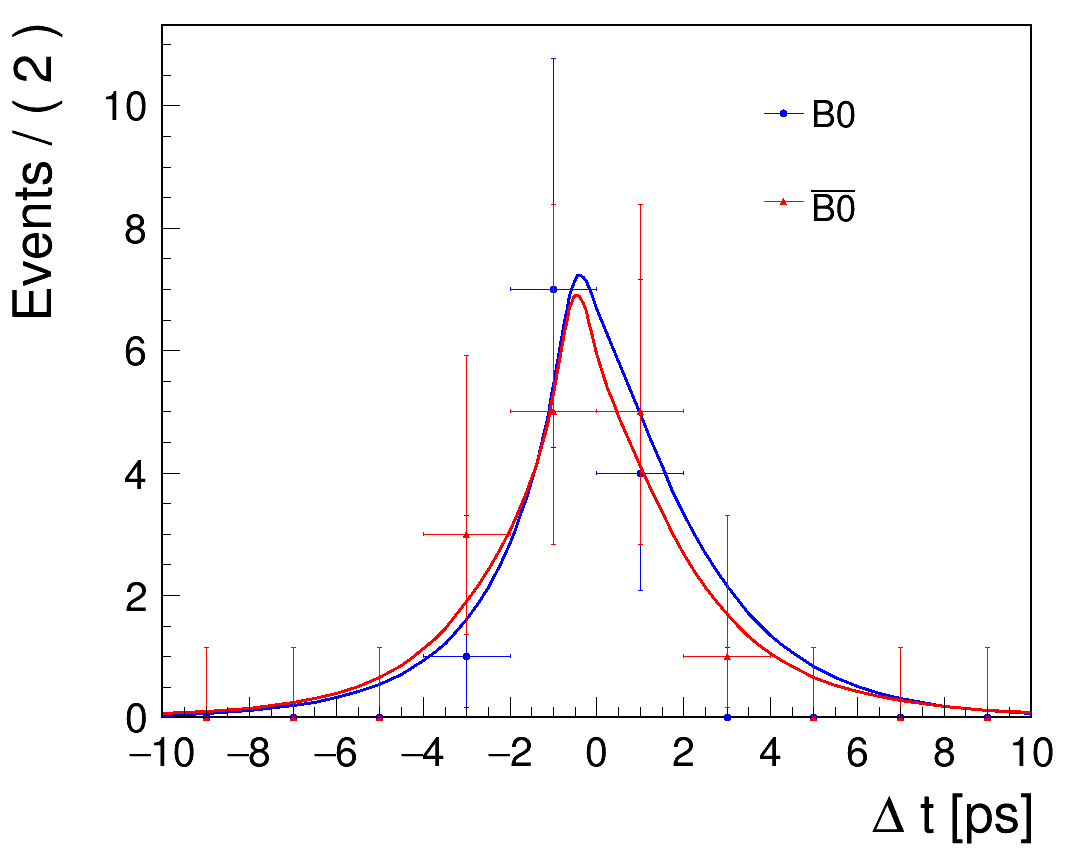
\includegraphics[height=5cm]{figures/cpfit-30gen}
		\caption{$\it{CP}$ fit on 30 \textit{generic MC}.}
		\label{fig:cpfit_gen_data}
	\end{minipage}
\end{figure}


\begin{table}
	\centering
	\caption{The $\it{CP}$ fit results using \textit{signal MC} and \textit{generic MC} with only statistical uncertainties.}
	\label{tab:cpfit_result_mc}
\begin{tabular}{|c|c|c|}
	\hline
	Sample (events)& $\mathcal{S}$ &  $\mathcal{A}$\\
	\hline
	\textit{signal MC} (8873) & sin$(2\phi_1) = 0.00 \pm 0.04 $ &  $\mathcal{A} = -0.01 \pm 0.02$\\
	\hline
	\textit{generic MC} (373) &  sin$(2\phi_1)  = 0.00 \pm 0.21$ & $\mathcal{A}  = -0.05 \pm 0.07$ \\
	\hline
	\textit{generic MC} (30) & sin$(2\phi_1) = 0.20 \pm 0.85 $& $\mathcal{A} = -0.06 \pm 0.30$ \\
	\hline
\end{tabular}
\end{table}
\begin{comment}
The fit result for 8873 signal MC is:
\begin{equation}
\begin{split}
sin(2\phi_1) & = 0.00 \pm 0.04 \\
\mathcal{A} & = -0.01 \pm 0.02\\
\end{split}
\end{equation} 
the fit result for 373 generic MC is:
\begin{equation}
\begin{split}
sin(2\phi_1) & = 0.00 \pm 0.21 \\
\mathcal{A} & = -0.05 \pm 0.07\\
\end{split}
\end{equation} 
the fit result for 30 events generic MC is:
\begin{equation}
\begin{split}
sin(2\phi_1) & = 0.20 \pm 0.85 \\
\mathcal{A} & = -0.06 \pm 0.30\\
\end{split}
\end{equation} 
\end{comment}

The fit results are consistent with expectation in non-$\it{CP}$ violation from MC input, and the statistical uncertainties has the tendency $\delta \propto 1/\sqrt{N}$ as poission distribution, where $N$ is events number used for $\it{CP}$ fit. To test fit on non-zero $\it{CP}$ violating MC, the fit on $B^0\to J/\psi K_S^0$ \textit{signal MC} is also done, the details of events selection as well as fit model determination can be found\cite{jpsiks_ichep}. The fit result over 10000 events is shown in Figure \ref{fig:cpfit_jpsiks}, which results in sin$(2\phi_1) = 0.70 \pm 0.05 $ and $\mathcal{A} = -0.01\pm 0.02$. The results agree with the input.
\begin{figure}[H]
	\centering
	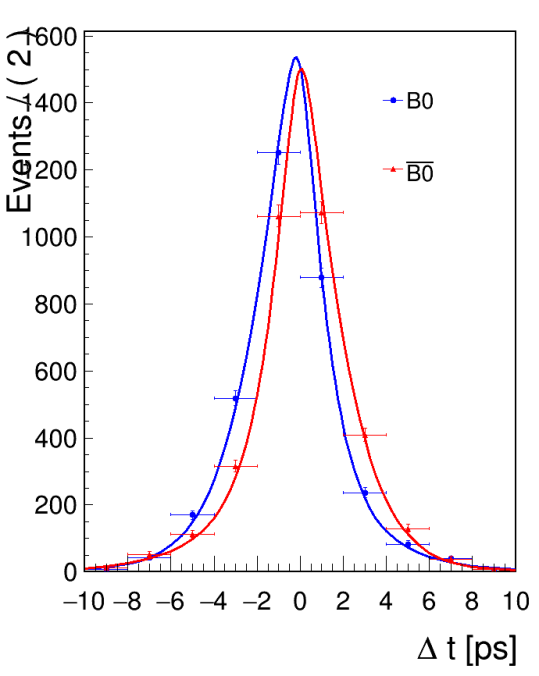
\includegraphics[height=5cm,width=6cm]{figures/jpsiks_cpfit10000}
	\caption{$\it{CP}$ fit over 10000 $B^0\to J/\psi K_S^0$ \textit{signal MC}. }
	\label{fig:cpfit_jpsiks}
\end{figure}
%We test the $\it{CP}$ fit on the sideband data with $M_{bc} < 5.27$ GeV.

\subsection{Linearity Test}
To validate the $\it{CP}$ fit linearity, a series of toy MC samples is generated, which the $\chi^2$ from vertex fit, events number $N$ and vertex errors on $\it{CP}$ and tag-side are sampled from the distribution of \textit{signal MC}. The resolution functions parameters are kept as same as $\it{CP}$ fit on \textit{generic MC}. The input $\mathcal{A}$ is set to zero while the input value of sin$(2\phi_1)$ is running from 0.1 to 0.9. Each dataset contains 10000 events. The dependence between input and output are shown in Figure \ref{fig:cpfit_line_S}. The linearity fit shows a good agreement between input and output.

\begin{figure}[H]
	\begin{minipage}{0.5\linewidth}
		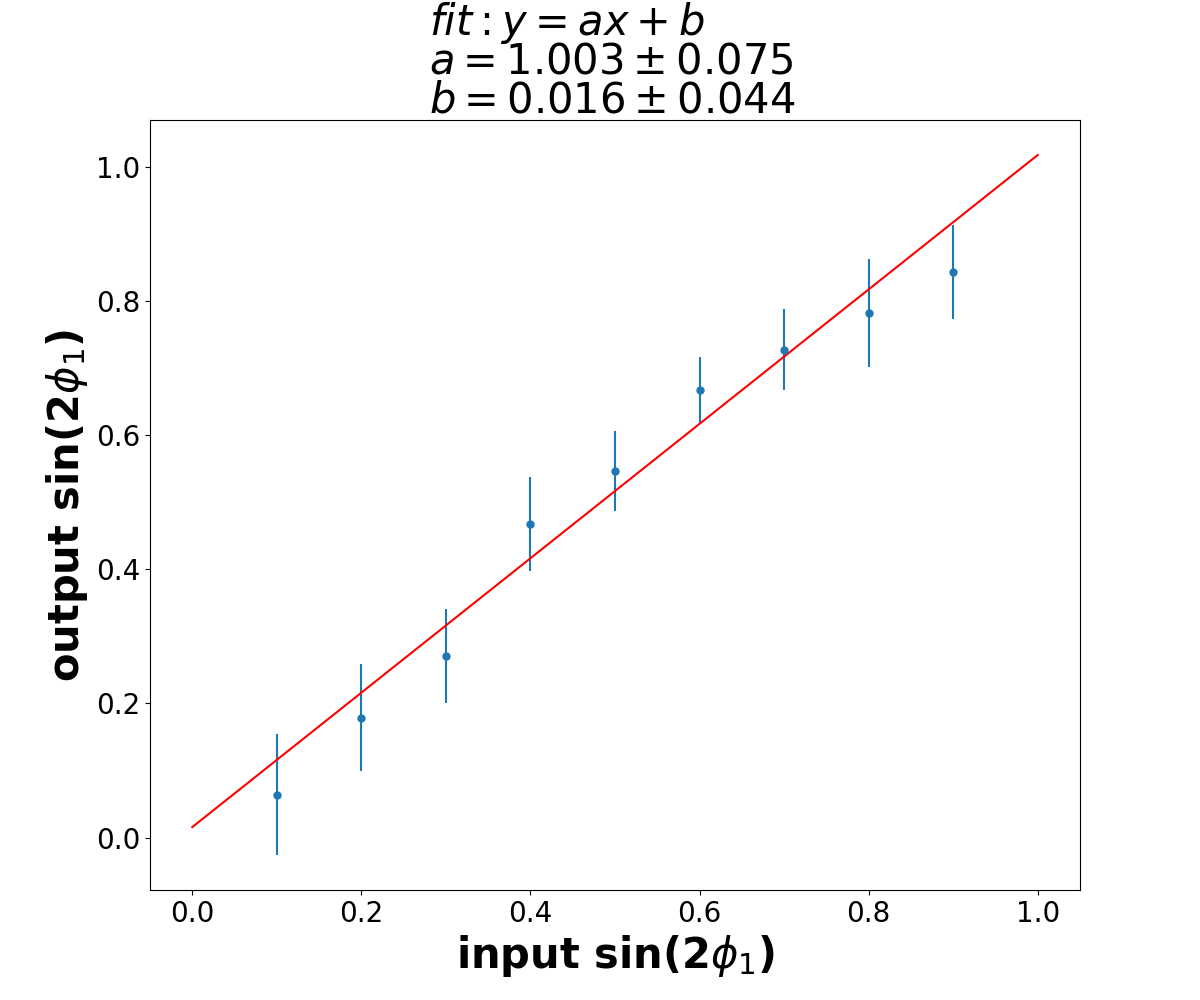
\includegraphics[height=6cm]{figures/S-test-line}
		%\caption{$\it{CP}$ fit on 8873 signal MC.}
	\end{minipage}
	\begin{minipage}{0.5\linewidth}
		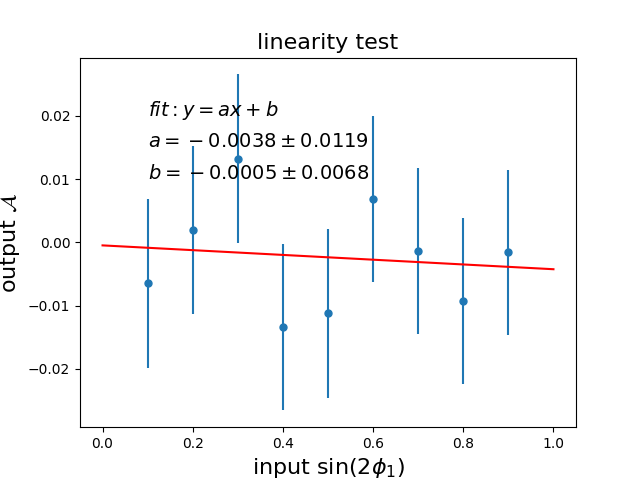
\includegraphics[height=6cm]{figures/A-test-line}
		%\caption{$\it{CP}$ fit on 373 generic MC.}
	\end{minipage}
	\caption{Linearity test of $\it{CP}$ fit.}
	\label{fig:cpfit_line_S}
\end{figure}

Also, we fix sin$(2\phi_1)$ at zero while floating $\mathcal{A}$ from  0.1 to 0.9, the dependence between input and output are as Figure \ref{fig:cpfit_line_A} shows. The linearity fit shows a good agreement as well.
\begin{figure}[H]
	\begin{minipage}{0.5\linewidth}
		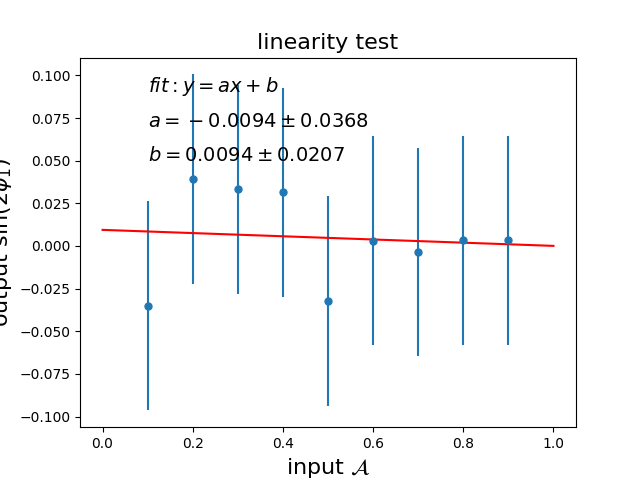
\includegraphics[height=6cm]{figures/S-test-line_fixS}
		%\caption{$\it{CP}$ fit on 8873 signal MC.}
	\end{minipage}
	\begin{minipage}{0.5\linewidth}
		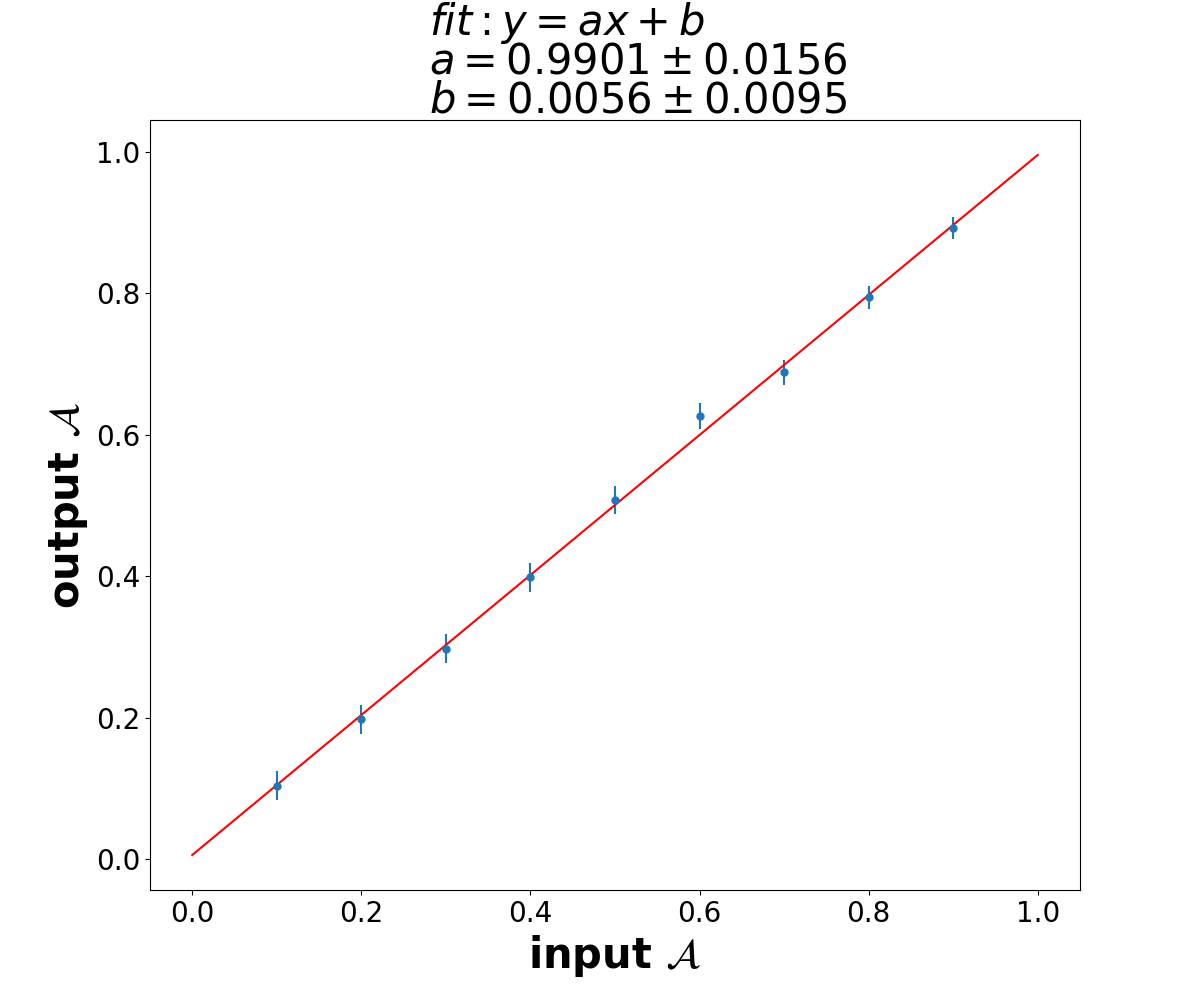
\includegraphics[height=6cm]{figures/A-test-line_fixS}
		%\caption{$\it{CP}$ fit on 373 generic MC.}
	\end{minipage}
	\caption{Linearity test of $\it{CP}$ fit.}
	\label{fig:cpfit_line_A}
\end{figure}

\subsection{Toy MC Fit Pull}
In order to check the fit bias with input-output method, a series of 1000 dataset of toy MC has been created containing about 26 events in each. The event number is set based on the expected number from signal region in data after the selection. The $\chi^2$ from vertext fit, events number $N$ and vertex errors on $\it{CP}$ and tag-side are sampled from the distribution of data. The fit to dataset is performed with zero input sin(2$\phi_1$) and $\mathcal{A}$ as floating parameters.
We expect to use the normal distribution to fit the pull of sin(2$\phi_1$) and $\mathcal{A}$. 

\begin{figure}[H]
	\begin{minipage}{0.5\linewidth}
		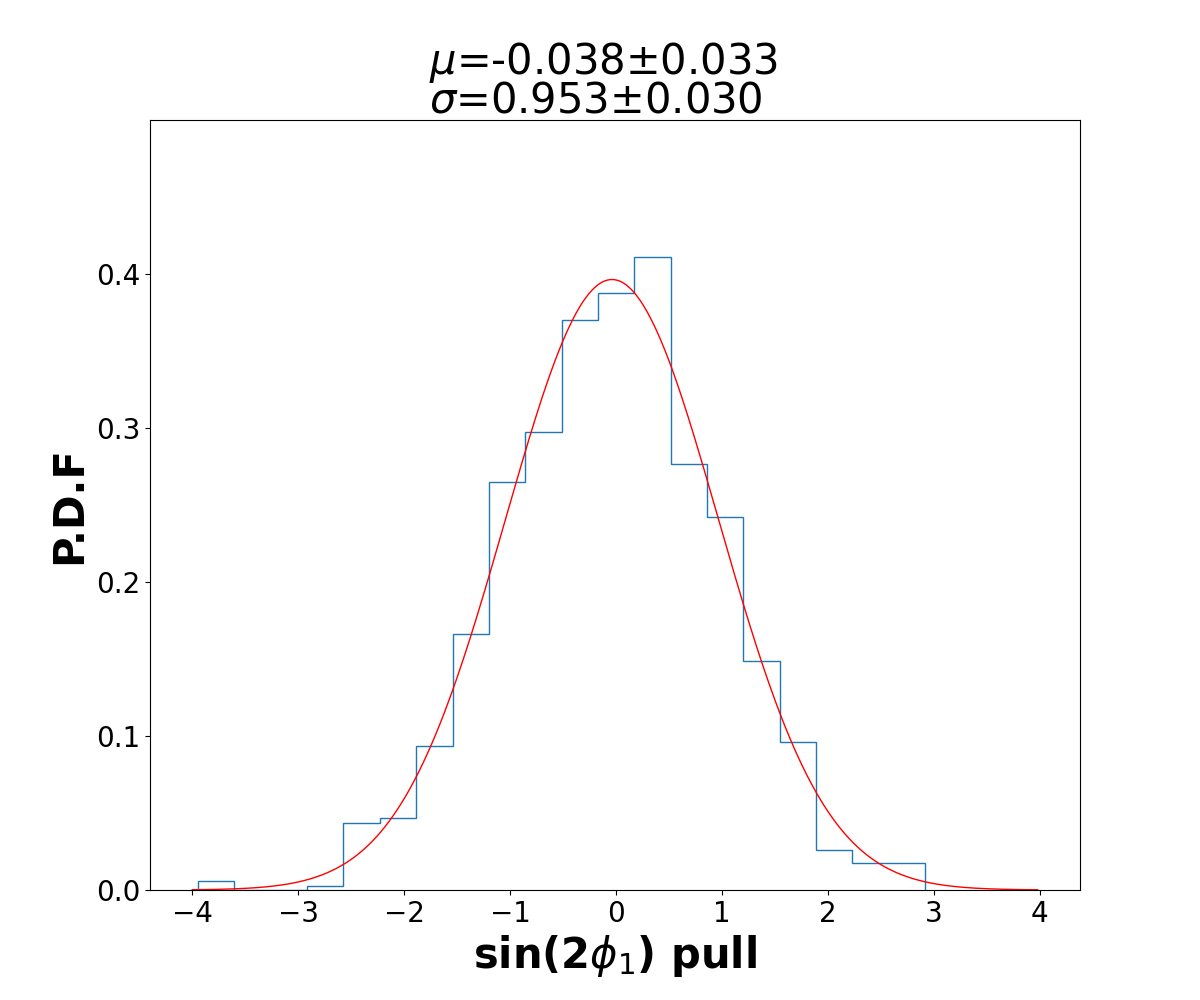
\includegraphics[height=6cm]{figures/pull_hist_S}
		%\caption{$\it{CP}$ fit on 8873 signal MC.}
	\end{minipage}
	\begin{minipage}{0.5\linewidth}
		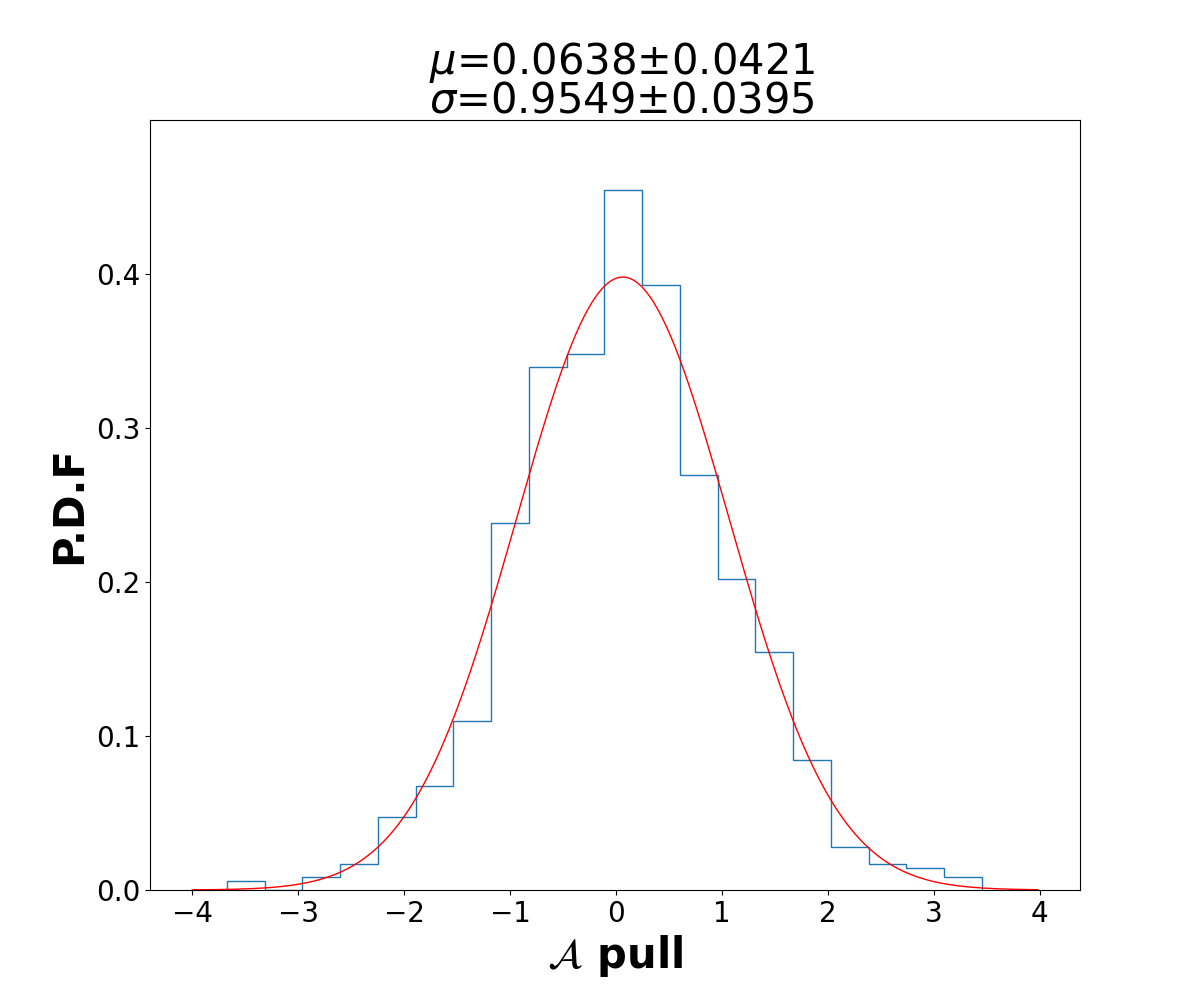
\includegraphics[height=6cm]{figures/pull_hist_A}
		%\caption{$\it{CP}$ fit on 373 generic MC.}
	\end{minipage}
	\caption{Pull of sin$(2\phi_1)$ and $\mathcal{A}$ fitted with the standard normal distribution.}
\end{figure}

The fit results shows a good recovery of input sin$(2\phi_1)$ and $\mathcal{A}$ with no clear bias is spotted.


\subsection{Lifetime and $\Delta m_d$ Fit}
Before looking at $\it{CP}$ parameters in data, we need to check if the physics parameters are consistent when setting the $\it{CP}$ fitter to fit them in float. To test lifetime fit, first we use 10000 \textit{signal MC} events which is generated by $\tau_{B^0} = 1.520$ from PDG value. The sin$(2\phi_1)$ and $\mathcal{A}$ are fixed at zero during the fit, for which the generator level $\it{CP}$ violation is zero. This is equivalent fit to Equation \ref{eq:cpfit_mc_life}.
\begin{equation}\label{eq:cpfit_mc_life}
\mathcal{P}(\Delta t,\tau_{B^0}) = 
\frac{e^{-|\Delta t|/\tau_{B^0}}}{4\tau_{B^0}}
\end{equation}
The fit result on \textit{signal MC} is $1.537 \pm 0.024$ ps which is consistent with the input. We perform the lifetime fit on data in signal region, and the $\it{CP}$ parameters are fixed based on PDG values to: sin$(2\phi_1)=0.69$ and $\mathcal{A} = 0$. The fitted lifetime from $B^0 \to K_S^0  K_S^0  K_S^0$ is $1.431\pm 0.382$ ps. The result is consistent with PDG value. The distribution of $\Delta t$ in lifetime fit is shown as Figure \ref{fig:cpfit_data_life}.
The $B^0$ and $B^+$ lifetime fit using control sample is also performed and summarized in here\cite{jpsiks_ichep}. The results are consistent with PDG values as input in MC generator. 
\begin{figure}[H]
	\centering
	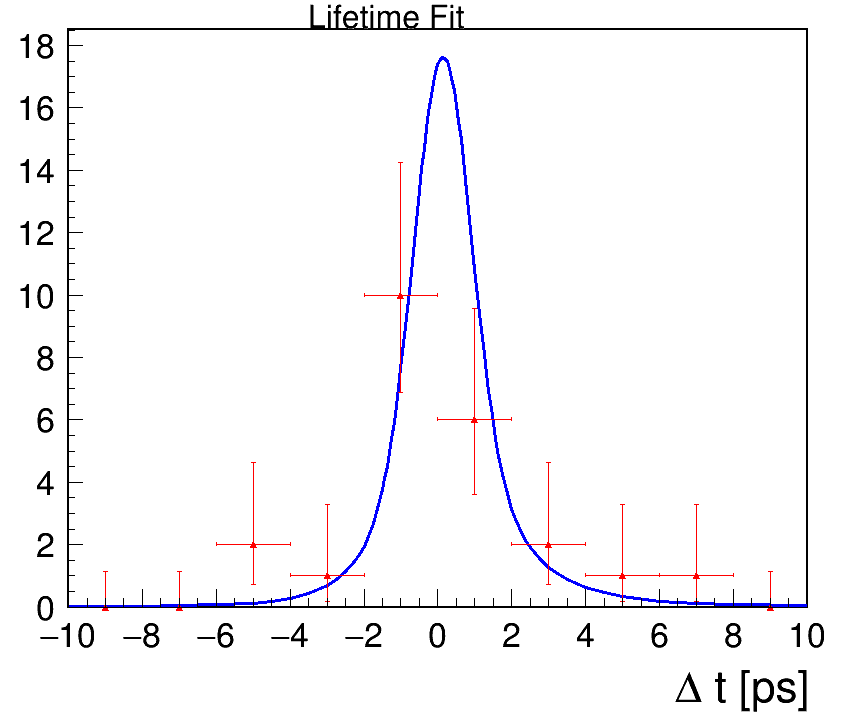
\includegraphics[height=7cm]{figures/lifetime_data}
	\caption{Lifetime fit on data}
	\label{fig:cpfit_data_life}
\end{figure}
%\subsection{Control Sample fit}

To test the fit on physics parameter $\Delta m_d$, we generate 200 toy MC sets of $B^0 \to K_S^0  K_S^0  K_S^0$ with input $\Delta m_d = 0.507 $ GeV/$c^2$ where each set contains 26 events as same as data. The fit result is close to normal distribution and the pull of $\Delta m_d$ is shown in Figure \ref{fig:cpfit_dm_pull}. 
\begin{figure}[H]
	\centering
	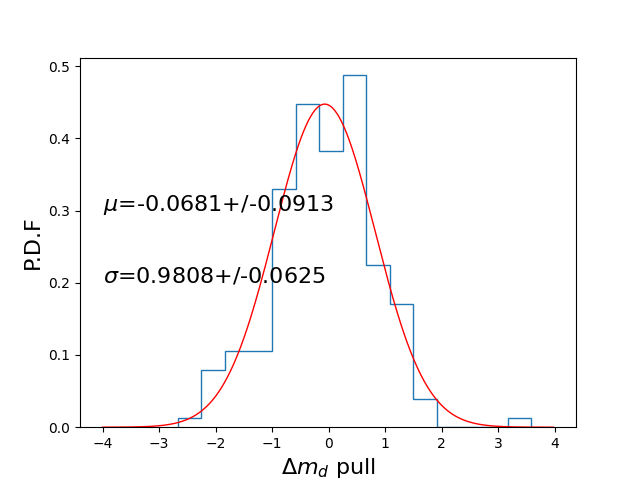
\includegraphics[height=7cm]{figures/pull_hist_dm}
	\caption{Pull of $\Delta m_d$}
	\label{fig:cpfit_dm_pull}
\end{figure}
%\subsection{Control Sample fit}

\section{$\it{CP}$ fit on data}
After the $\it{CP}$ fit procedures are reviewed by Belle II collaboration, the permission of measuring $\it{CP}$ parameters using 62.8 fb$^{-1}$ Belle II data is granted. The events number used for the $\it{CP}$ fit is 26, and the fit result is shown Figure \ref{fig:cpfit_data}.

\begin{figure}[H]
	\centering
	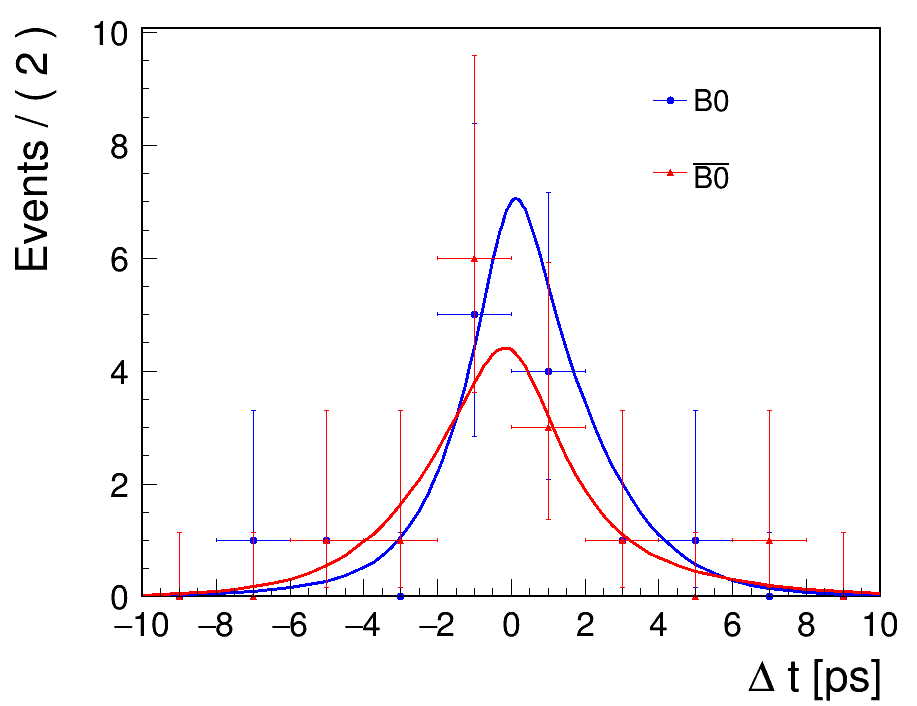
\includegraphics[height=6cm]{cpfit-data}
	\caption{The $\it{CP}$ fit from data.}
	\label{fig:cpfit_data}
\end{figure}

The results of $\it{CP}$ parameters are: 

\begin{equation}
\begin{split}
sin(2\phi_1) & = 0.82 \pm 0.85(stat) \\
\mathcal{A} & = -0.21 \pm 0.28(stat) \\
\end{split}
\end{equation} 

\section{Systematic Uncertainty}
The systematic uncertainty that affects the fit results may come from many aspects of the measurement setup. The contributions at the curent stage of Belle II are summarized as Table \ref{tab:sy_sub}.
For the listed sources of systematic uncertainty, if the parameters are defined with MC study, we float the value by $\pm 2 \sigma$, and if the parameters are defined by data, we float the value by $\pm 1 \sigma$, where $\sigma$ is the uncertainty of the parameters. The impact of $\it{CP}$ parameters are separately estimated from each sources with positive and negative differentials. By adding in quadrature of each term, the sub-total contributions and the overall systematic uncertainty are obtained. 
\begin{table}
	\centering
	\begin{tabular}{c|c|c} 
		\hline
		Sources &  $\delta \mathcal{S}$ & $\delta \mathcal{A}$\\
		\hline
		signal fraction  & 0.044387 & 0.033932 \\
		background $\Delta t$ shapes & 0.039430 & 0.037269\\
		signal $\Delta t$ shapes & 0.033671 & 0.009283 \\
		wrong tag fraction & 0.003709 & 0.003790\\
		fit bias & 0.009817 & 0.005702 \\
		physics parameters & 0.006923 & 0.001250\\ 
		\textit{KsFinder} impact on data & 0.004852 & 0.000606\\
		vertex reconstruction & 0.019007 & 0.020563\\
		\hline
		Total & 0.072121 & 0.055661\\
		\hline
	\end{tabular}
	\caption{The contributions of each source of systematic uncertainty.}
	\label{tab:sy_sub}
\end{table}
\begin{comment}
\begin{itemize}
\item resolution functions parameters
\item signal fraction
\item flavor tagging 
\item background $\Delta t$ shapes
\item fit bias
\item physics parameters
\item KsFinder impact on data
\item vertex reconstruction
\end{itemize}
\end{comment}

The signal resolution functions' parameters are determined from MC study for signal component. The impact on fit results is summarized as follows Table \ref{tab:sy_sigt}.
\begin{table}[H]
	\begin{minipage}[b]{1.0\linewidth}
		\centering
		\caption{systematic uncertainty from signal $\Delta t$ shapes}
		\label{tab:sy_sigt}
		\begin{tabular}{c r r r r}
			\hline
			source & $+\delta \mathcal{S}$ & $+\delta \mathcal{A}$ & $-\delta \mathcal{S}$ &  $-\delta \mathcal{A}$\\
			\hline
			$f_{cp}^{tail}$ & -0.000096 & -0.000057
			& 0.000014
			& 0.000056
			\\
			$s_0^{main}$& 0.005443
			& 0.001299
			& -0.005675
			& -0.001404
			\\
			$s_1^{main}$ & 0.019934
			& -0.000903
			& -0.020204
			& 0.000633
			\\
			$s_0^{tail}$ &  -0.003233
			& -0.001623
			& 0.003270
			& 0.001596
			\\
			$f_{tag}^{tail}$ & 0.003140
			& -0.001257
			& -0.003117
			& 0.001266
			\\
			$s_0^{main}$&  0.002011
			& -0.001395
			& -0.001956
			& 0.001398
			\\
			$s_1^{main}$ & 0.005059
			& -0.000840
			& -0.004969
			& 0.000825
			\\
			$s_0^{tail}$ &  -0.000135
			& -0.000393
			& 0.000101 & 0.000435
			\\
			$s_1^{tail}$  & 0.000101 & 0.000027 &  -0.000472
			& 0.000129
			\\
			$f_{\delta}$ & -0.007248
			& -0.000552
			& 0.007231
			& 0.000591
			\\
			$f_p$ &  0.003037
			& 0.004347
			& -0.003069
			& -0.004314
			\\
			$\tau_n$ & -0.001010 & -0.002841
			& 0.000937
			& 0.002940
			\\
			$\tau_p$ &  0.004497
			& 0.002502
			& -0.004648
			& -0.002478
			\\
			\hline
			Total &
			\multicolumn{2}{c}{$\delta \mathcal{S}=0.033671$} &
			\multicolumn{2}{c}{$\delta \mathcal{A}=0.009283$}\\
			\hline
		\end{tabular}
	\end{minipage}
\end{table}
The background $\Delta t$ shapes' parameters are determined from data sideband $M_{bc}<5.26$ GeV. The impact on fit results is summarized in Table \ref{tab:sy_bkgt}.
\begin{table}[H]
	\begin{minipage}[b]{1.0\linewidth}
		\centering
		\caption{systematic uncertainty from background $\Delta t$ shapes}
		\label{tab:sy_bkgt}
		\begin{tabular}{c r r r r}
			\hline
			source & $+\delta \mathcal{S}$ & $+\delta \mathcal{A}$ & $-\delta \mathcal{S}$ &  $-\delta \mathcal{A}$\\
			$\mu^{bkg}_{\delta}$ & -0.014294
			& -0.016581
			& 0.006758
			& 0.006537
			\\
			$\mu^{bkg}_{l}$&  -0.002798
			& -0.012567
			& 0.003789
			& 0.012783
			\\
			$\tau_{bkg}$ & 0.001377
			& 0.001689
			& -0.004159
			& 0.000085\\
			$f_{\delta}^{bkg}$ &  -0.011315
			& 0.001365
			& 0.011187
			& -0.001395
			\\
			$f^{bkg}_{tail}$  &-0.002661
			& 0.001530
			& 0.002480
			& -0.001368
			\\
			$\sigma^{bkg}_{main}$ & 0.020702
			& 0.022041
			& -0.023618
			& -0.015690
			\\
			$\sigma^{bkg}_{tail}$ & -0.000275 & -0.000159
			& 0.000179
			& 0.000141
			\\
			\hline
			Total &
			\multicolumn{2}{c}{$\delta \mathcal{S}=0.039430$} &
			\multicolumn{2}{c}{$\delta \mathcal{A}=0.037269$}\\
			\hline
		\end{tabular}
	\end{minipage}
\end{table}
The flavor tagging parameters wrong tagging fraction $ w$ in each rbin is determined from control sample. The impact in each rbin on fit results is summarized in Table \ref{tab:sy_wtag}: 
\begin{table}[H]
	\begin{minipage}[b]{1.0\linewidth}
		\centering
		\caption{systematic uncertainty from wrong tagging fraction}
		\label{tab:sy_wtag}
		\begin{tabular}{c r r r r}
			\hline
			source & $+\delta \mathcal{S}$ & $+\delta \mathcal{A}$ & $-\delta \mathcal{S}$ &  $-\delta \mathcal{A}$\\
			$w_1$ & -0.001892
			& 0.001911
			& 0.001855
			& -0.002004
			\\
			$ w_2$ & -0.001645
			& 0.001104
			& 0.001609
			& -0.001155
			\\
			$ w_3$ & -0.000490
			& 0.001344
			& 0.000473
			& -0.001341
			\\
			$ w_4$ & 0.000656
			& 0.000264
			& -0.000654
			& -0.000255 \\
			$ w_5$ & -0.000123
			& 0.000204
			& 0.000123 &
			-0.000195
			\\
			$ w_6$ & 0.000095 & 0.000054 & 0.000096 & -0.000045 \\
			$ w_7$ & 0.000191
			& -0.000396
			& -0.000191
			& 0.000402
			\\
			\hline
			Total &
			\multicolumn{2}{c}{$\delta \mathcal{S}=0.003709$} &
			\multicolumn{2}{c}{$\delta \mathcal{A}=0.003790$}\\
			\hline
		\end{tabular}
	\end{minipage}
\end{table}
The physics parameters $\Delta m_d$ and $\tau_{B^0}$ uncertainties are included using the PDG average value. The impact on fit results is summarized in Table \ref{tab:sy_phys}.
\begin{table}[H]
	\begin{minipage}[b]{1.0\linewidth}
		\centering
		\caption{systematic uncertainty from  physics parameters}
		\label{tab:sy_phys}
		\begin{tabular}{c r r r r}
			\hline
			source & $+\delta \mathcal{S}$ & $+\delta \mathcal{A}$ & $-\delta \mathcal{S}$ &  $-\delta \mathcal{A}$\\
			$\Delta m_d$  & -0.001767
			& -0.000687
			& 0.001778
			& 0.000696
			\\
			$\tau_{B^0}$  & -0.004561
			& -0.000546
			& 0.004565
			& 0.000555
			\\
			\hline
			Total &
			\multicolumn{2}{c}{$\delta \mathcal{S}=0.006923$} &
			\multicolumn{2}{c}{$\delta \mathcal{A}=0.001250$}\\
			\hline
		\end{tabular}
	\end{minipage}
\end{table}
The signal fraction is determined using 2D fit results of $M_{bc}$ and $\Delta E$ from data. The impact on fit results is summarized in Table \ref{tab:sy_fsig}.
\begin{table}[H]
	\begin{minipage}[b]{1.0\linewidth}
		\centering
		\caption{systematic uncertainty from  signal fraction}
		\label{tab:sy_fsig}
		\begin{tabular}{c r r r r}
			\hline
			source & $+\delta \mathcal{S}$ & $+\delta \mathcal{A}$ & $-\delta \mathcal{S}$ &  $-\delta \mathcal{A}$\\
			mu1\_mbc  & 0.000822 &	-0.003888&	-0.000797&	0.003849
			\\
			sigma1\_mbc & 0.000476 &	0.008442&	-0.000628&	-0.008733
			\\
			m0\_argus & -0.000707&	0.004140	&0.001448&	-0.005781
			\\
			c\_argus & -0.005544&	0.001449&	0.000922&	-0.000078\\
			f1\_de & 0.027826 &	0.020589&	-0.019237	&-0.008409
			\\
			f2\_de & 0.020809&	0.017649	&-0.016129	&-0.007005
			\\
			mu1\_de & -0.000443&	-0.000153&	0.000496&	0.000088\\
			mu2\_de & -0.000563&	0.001446&	0.000591&	-0.001446
			\\
			mu3\_de & -0.003164&	-0.000834&	0.003354&	0.000981
			\\
			sigma1\_de& -0.000172&	-0.000966&	0.000206&	0.000906
			\\
			sigma2\_de& -0.003150&	0.002958&	0.002635&	-0.002475
			\\
			sigma3\_de& -0.001926&	-0.002550&	0.002470&	0.002985
			\\
			a0\_cheb & 0.000952&	0.000057&	-0.000893&	-0.000102
			\\
			N\_sig\_f & -0.004640&	0.003987&	0.004922&	-0.003504
			\\
			\hline
			Total &
			\multicolumn{2}{c}{$\delta \mathcal{S}=0.044387$} &
			\multicolumn{2}{c}{$\delta \mathcal{A}=0.033932$}\\
			\hline
		\end{tabular}
	\end{minipage}
\end{table}

The fit bias uncertainties is determined by taking the larger ones among the fit error of 300000 \textit{signal MC}  events  with zero $\it{CP}$ violation and the difference between input and output of the center value. The fit result is $\mathcal{S} = 0.000127\pm0.009817$ and $\mathcal{A} = 0.000265\pm0.005702$. So the values of fit errors are used as listed in Table \ref{tab:fitbias}.
\begin{table}[H]
	\begin{minipage}[b]{1.0\linewidth}
		\centering
		\caption{systematic uncertainty from fit bias}
		\label{tab:fitbias}
		\begin{tabular}{c c c}
			\hline
			source & $\delta \mathcal{S}$ & $\delta \mathcal{A}$ \\
			fit bias & 0.009817 & 0.005702\\
			\hline
		\end{tabular}
	\end{minipage}
\end{table}

Applying KsFinder cut at 0.74 based on MC study may introduce small impact on data due to the different response on the classifier between data and MC. Therefore the contribution of systematic uncertainty from KsFinder is considered. At cut value  0.74, the $\mathcal{R_{B^0}}$ presenting MC and data signal yield ratio is $\mathcal{R}_{B^0} = 1.027 \pm 0.033$, where the upper and lower limit is 1.060 and 0.994, respectively. These two ratios are applied on the signal fraction obtained by data to repeat the fit, and the difference of fit results compared to the original values are used as systematic uncertainty, see Table \ref{tab:sy_ks}.

\begin{table}[H]
	\begin{minipage}[b]{1.0\linewidth}
		\centering
		\caption{systematic uncertainty from KsFinder.}
		\label{tab:sy_ks}
		\begin{tabular}{c r r}
			\hline
			source & $\delta \mathcal{S}$ & $\delta \mathcal{A}$ \\
			$\mathcal{R}_{B^0}=1.06$ & 0.004826
 & -0.000606\\
			$\mathcal{R}_{B^0}=0.994$ & -0.000508
& 0.000007
\\
			\hline
			Total &
			{$0.004852$} &
			{$0.000606$}\\
			\hline
		\end{tabular}
	\end{minipage}
\end{table}

For the contributions from vertex reconstruction, the impacts from the selections in Table \ref{tab:cutCP} are considered. Given the fact that cut values in Table \ref{tab:cutCP} are very loose and the statistics from data is very limited, the changing of the these values doesn't affect events collected from data so that systematic uncertainty can not be reflected correctly. Therefore, 1 ab$^{-1}$ \textit{generic MC} is used with the modified ranges to estimate the potential systematic uncertainty from vertex reconstruction. Besides, due to the absence of IP constraint in vertex fit, the impact from the IP constraint options as well as the potential bias are not considered. The summarized systematic uncertainties are listed in Table \ref{tab:sy_vertex}, where the zero values appear due to the unchanged events input under the modified ranges.

\begin{table}[htpb]
	\begin{minipage}[b]{1.0\linewidth}
		\centering
		\caption{systematic uncertainty from vertex reconstruction}
		\label{tab:sy_vertex}
		\begin{tabular}{c r r}
			\hline
			source & $\delta \mathcal{S}$ & $\delta \mathcal{A}$ \\
			$\sigma_{z_{tag}}<0.05$ cm & 0.004369
& -0.003599
\\
			$\sigma_{z_{tag}}<0.15$ cm & 0.000000 & 0.000000 \\
			$\chi^2/N(CP)<3$ & 0.018197
& -0.020242
\\
			$\chi^2/N(CP)<13$ & 0.000000 & 0.000000\\
			$\chi^2/N(tag)<40$ & 0.000000
& 0.000000
\\
			$\chi^2/N(tag)<60$ & 0.000000 & 0.000000\\
			$|\Delta t|<50 $ ps & 0.003325
& -0.000396
\\
			$|\Delta t|<90 $ ps & 0.000000 & 0.000000\\
			IP constraint & 0.000000& 0.000000\\
						\hline
							Total &
						{$0.019007$} &
						{$0.020563$}\\
						\hline
		\end{tabular}
	\end{minipage}
\end{table}

